\chapter{Index Maintenance}

\section{Introduction}
\label{sec:intro}

% Web archives

In recent years, there has been an increasing awareness that
born-digital contents, such as those on the Web, are ephemeral but
often worth preserving. Organizations involved in the preservation of
web contents include non-profits (e.g., the Internet Archive~\cite{ia}
and the Internet Memory Foundation~\cite{imf}), for-profit companies,
as well as national libraries and universities. The motivations behind
such web archives are diverse and range from preservation of cultural
heritage to compliance with legal requirements.

% Time-travel text search

Web archives typically contain multiple versions of every document
that reflect the evolution of its content over time. Interfaces
provided to users in order to access archived contents, though, are
still limited, for instance, to URL-based lookup \& browsing as in the
Internet Archive's Wayback Machine or simple keyword search. Motivated
by this, \textit{time-travel text search} has been proposed as an
extension of standard text search by temporal predicates. Users can
thus combine a keyword query (e.g., \textsf{financial crisis}) with a
time interval (e.g., \texttt{\small [2006, 2008]}) to retrieve all
document versions from the archive that are considered relevant to the
given keywords and existed during the given time interval. Different
index structures~\cite{aanand:cikm2010,
  aanand:sigir2011,kberberi:sigir2007} have been proposed to
efficiently support time-travel text search, incurring controllable
overhead either in terms of index size or response time when compared
to standard text search.

% No updates

However, none of the existing index structures for time-travel text
search can easily be updated when additional document versions are
archived. To keep up with the state of the web archive, they thus have
to be rebuilt periodically. While this used to be the case as well for
standard inverted indexes, their maintenance in the presence of
\textit{insertions}, \textit{modifications}, and \textit{deletions} of
documents is now fairly
well-understood~\cite{Buttcher:2008fk,Lester:2006ly,Peng:2010fk}.

% Separation

Our approach put forward in this work efficiently supports time-travel
text search and handles additions of new document versions to the
archive. It distinguishes between \textit{active versions}, as the
most recent and still current document versions, and \textit{archive
  versions}, as the document versions already superseded by a more
recent version of the same document. To search the active versions, a
standard incrementally updatable inverted
index~\cite{Buttcher:2008fk,Lester:2008qf} is employed, which we will
not discuss further. Our focus instead is on searching the archive
versions. We propose a novel index structure to this end, building on
our own sharded index for time-travel text
search~\cite{aanand:sigir2011}, and describe how it can be maintained
incrementally when document versions are superseded and thus need to
be migrated from the active index.

The original sharded index for time-travel text search relies on a
method to horizontally partition each index list, so that any
time-travel query can be processed without sequentially reading index
entries that do not overlap with the query time-interval. It then
relaxes the horizontal partitions determined (the so-called
\textit{shards}), taking into account the I/O characteristics of the
storage infrastructure, encoded as a parameter $\eta$ reflecting the
cost ratio between random seeks and sequential reads. The method
guarantees for every \textit{relaxed shard} that the \textit{expected
  number} of wastefully read index entries is bounded by $\eta$. We
are more stringent in this work and consider the worst case by
bounding the \textit{maximum number} of wastefully read index entries
instead. This allows us to develop an online incremental sharding
algorithm that keeps only a small in-memory buffer for every shard in
the archive index. We show that our online algorithm is within an
approximation factor of $(2 - \frac{2}{\eta + 2})$ and hence results
in at most two times the optimal number of relaxed shards.

We conducted experiments on the revision history of the English
Wikipedia and the UKGOV web archive, as two large-scale real-world
datasets. Our results show that incrementally maintaining our novel
index structure is an order of magnitude more efficient than
periodically rebuilding a sharded index for time-travel text
search. Query processing performance, in addition, is not adversely
affected and even improves in some cases. We therefore believe that
the proposed approach provides the best of both worlds -- update
ability and efficient query processing -- two key features needed when
searching web archives but missing so far.

% Organization

The rest of this paper unfolds as follows: Section~\ref{sec:model}
introduces our model and
notation. Section~\ref{sec:index-organization} recaps key ideas behind
the sharded index that we build upon. Section~\ref{sec:inc_sharding}
describes our incremental sharding method to maintain the
index. Section~\ref{sec:system} presents the overall architecture of
our system. Our experimental evaluation is the subject of
Section~\ref{sec:eval}. Finally, we relate to existing research in
Section~\ref{sec:related-work} and conclude in
Section~\ref{sec:conclusions}.

% Model
\section{Data and Query Model}
\label{sec:model}

We consider a collection $\mathcal{D}$ of versioned documents that
change over time.  Each document $d$ is uniquely identified by an
identifier $id_{d}$.  At time $t$, document $d$ may have an active
version $d^*$ and zero or more archive versions $\langle d^{{1}},
d^{{2}}, \ldots \rangle$.  Each (active or archive) version $d^i$ of
$d$ comes with a valid-time interval $I(d^{i}) =
[\;begin(d^{i}),\,end(d^{i})\;)$ that denotes when that version was
the active version of $d$; for $d^*$, $end(d^*)=\infty$ and $t\in
I(d^*)$. We furthermore assume that all the $I(d^i)$ are disjoint.

The active version of a document turns into an archive version when
the document is re-crawled and either a new active version is found or
the document was removed from the Web. In both cases, the end time of
the old version is set to the current time.

We consider time-travel queries over $\mathcal{D}$ that consist of a
set of terms $Q = \{q_{1},\ldots,\,q_{m}\}$ and a time interval
$[b_{Q},\,e_{Q}]$. When evaluated, this query retrieves the set of
document versions that satisfy the keyword query $Q$ and existed at
any time during the time interval $[b_{Q},\,e_{Q}]$.

% Index Organization

\section{Index Organization}
\label{sec:index-organization}

We now describe our index organization and briefly recap the sharded
index for time
-travel text search~\cite{aanand:sigir2011} that we
build upon in this work.

% Index Organisation
Our system distinguishes between \emph{active versions}, as those that
are the most recent and still current version of a document, and
\emph{archive versions}, as those that have already been superseded by
a more recent version of the same document. To search them, our system
employs separate indexes, coined \emph{active index} and \emph{archive
  index}.

% Inverted Index
Both our indexes are based on the established inverted
index~\cite{DBLP:journals/csur/ZobelM06} that associates each term
with an \emph{index list}. Each entry in the index list, $\langle
id_{d}, I(d^{i}), s \rangle$, consists of a document identifier
$id_{d}$, a valid-time interval, $I(d^{i}) = [ begin(d^{i}),
end(d^{i})]$, and a payload $s$. The specifics of the payload depend
on the retrieval model and the types of queries to be supported -- it
can be empty, a scalar value (e.g., capturing term frequency), or
include positional information. When no confusion arises, we simply
use $begin(p)$ and $end(p)$ of an index entry $p$ to refer to the
valid-time interval boundaries of the corresponding document version.

% How are queries processed?
Queries that only ask for current information contained in active
versions can be processed using only the active index, which
corresponds to the live index that search engines maintain on the
current Web. Time-travel queries that also ask for information from
the past contained in archive versions are processed using both the
active index and the archive index in combination.

% Active index organization (e.g., optimizations)
The active index is implemented as an incrementally updatable inverted
index~\cite{Buttcher:2008fk,Lester:2008qf}. Depending on the fraction
of time-travel queries among all queries posed to the system, index
lists in the active index can be organized to efficiently support
queries on active versions or time-travel queries. For the former,
index entries may be ordered by their document identifier to allow for
more efficient query processing, possibly together with additional
structures~\cite{DBLP:conf/cikm/BroderCHSZ03,DBLP:conf/sigir/DingS11,DBLP:journals/tois/MoffatZ96,DBLP:conf/sigir/StrohmanC07}. For
the latter, index entries may be ordered by the begin boundary of
their valid-time interval to support efficient filtering of too recent
document versions.

% Archive index organization (recap of SIGIR 2011)
The archive index is implemented as a sharded
index~\cite{aanand:sigir2011}, whose key ideas we now briefly
recap. The sharded index distributes entries in an index list over
disjoint partitions coined \emph{shards}. Entries within a shard are
ordered by the begin boundary of their valid-time interval. In
addition, each shard comes with an \emph{impact list} that maintains,
for every possible begin boundary $b_{Q}$ of a query time-interval,
the position of the earliest entry in the shard whose valid-time
interval contains the begin boundary $b_{Q}$. In practice, impact
lists can be represented compactly and kept in main memory, as
described~in~\cite{aanand:sigir2011}.

% Query processing
When processing a time-travel query, all shards for the query terms in
$Q$ are read from the position stored in their impact list for the
begin boundary $b_{Q}$ of the query time-interval, as opposed to, from
their beginning. Per shard this involves one random seek to get to the
indicated position followed by a number of sequential reads. One can
safely stop reading a shard once the first index entry with a begin
boundary larger than $e_{Q}$ has been seen. The query processing cost
thus depends on the number of shards, each of which is accessed with a
random seek, and the total number of index entries that are read
sequentially. Every method that assigns index entries to shards has to
consider these two factors.

We now describe how index entries can be assigned to shards so as to
optimize query processing cost. Since the assignment of index entries
to shards solely depends on their valid-time intervals, we describe it
as an interval-to-shard assignment problem and use the notions index
entry and interval interchangeably. Let us first introduce some basic
notation for intervals that we need in what follows. An interval $I_j$
is associated with a begin time $begin(I_j)$ and an end time
$end(I_j)$. We say that an interval $I_1$ subsumes an interval $I_2$
(for short: $I_1 \sqsupset I_2$), if:
$$
begin(I_2) > begin(I_1) \,\,\wedge\,\, end(I_2) < end(I_1)\;.
$$

An index entry is said to be a wasted read, if it is accessed during
query processing although its valid-time interval does not overlap
with the query time-interval. Such a wasted read may be caused when an
interval $I_1$ \emph{subsumes} another interval $I_2$ in the same
shard. Assuming that a shard contains only these two intervals, the
impact list entry for a begin boundary $b_{Q}$ of the query
time-interval after the end of $I_2$ will point to $I_1$ which is
stored before $I_2$, and $I_2$ will be read even though it does not
qualify as query result.

Since all shards for a term are accessed for any time-travel query
including the term, the cost incurred due to random seeks is
proportional to the number of shards per term. The cost for random
seeks and sequential reads can be traded-off with two extremes. On one
hand we can eliminate the cost for all but one random seek by having
only a single shard per term. On the other hand, we can eliminate
wasted reads altogether by creating idealized shards. \emph{Idealized
  sharding} avoids subsumption entirely, i.e., there are no two
intervals $I_1$ and $I_2$ with $I_1 \sqsupset I_2$ in a shard. The
minimal number of idealized shards for a given set of intervals can be
determined using a greedy algorithm, as described
in~\cite{aanand:sigir2011}.

The best performing solution is usually in between these two extremes,
taking into account the I/O characteristics of the storage
infrastructure housing the index. \emph{Cost-aware sharding} developed
in~\cite{aanand:sigir2011} systematically allows for interval
subsumptions, while minimizing the overall number of shards. It thus
trades some additional wasted sequential reads for a reduced number of
random seeks. The method minimizes the number of shards per index list
(and hence the number of random seeks) by systematically merging
idealized shards. It thereby ensures that the expected number of
wasted sequential reads per shard is below a threshold $\eta$ encoding
the cost ratio between random seeks and sequential reads.

% Incremental Sharding
\section{Incremental Sharding}
\label{sec:inc_sharding}

Incremental sharding takes into account the relative costs of random and sequential accesses by a more restrictive bound on the number of subsumptions for a given shard. It bounds the absolute number of subsumptions for a given shards. This is opposed to cost-aware sharding in~\cite{aanand:sigir2011} where the number of subsumptions per shard were on an average limited to a system-wide parameter. A bound on the number of subsumptions per shard translates to bounding the number of sequential wasted reads. We term this restriction as the \emph{bounded subsumption} property. A shard is said to exhibit a bounded subsumption property if an interval in that shard does not subsume more than $\eta$ intervals, where $\eta$ is a system-wide constant same as before. Formally,

%We use a constraint which is similar yet slightly restrictive by bounding the number of subsumptions for an interval in a shard. We term this as the \emph{Bounded Subsumption} property. A shard is said to exhibit a bounded subsumption property if an interval in that shard does not subsume more $\eta$ intervals, where $\eta$ is a system-wide constant. Formally,
\begin{figure}[tb]
	\centering
		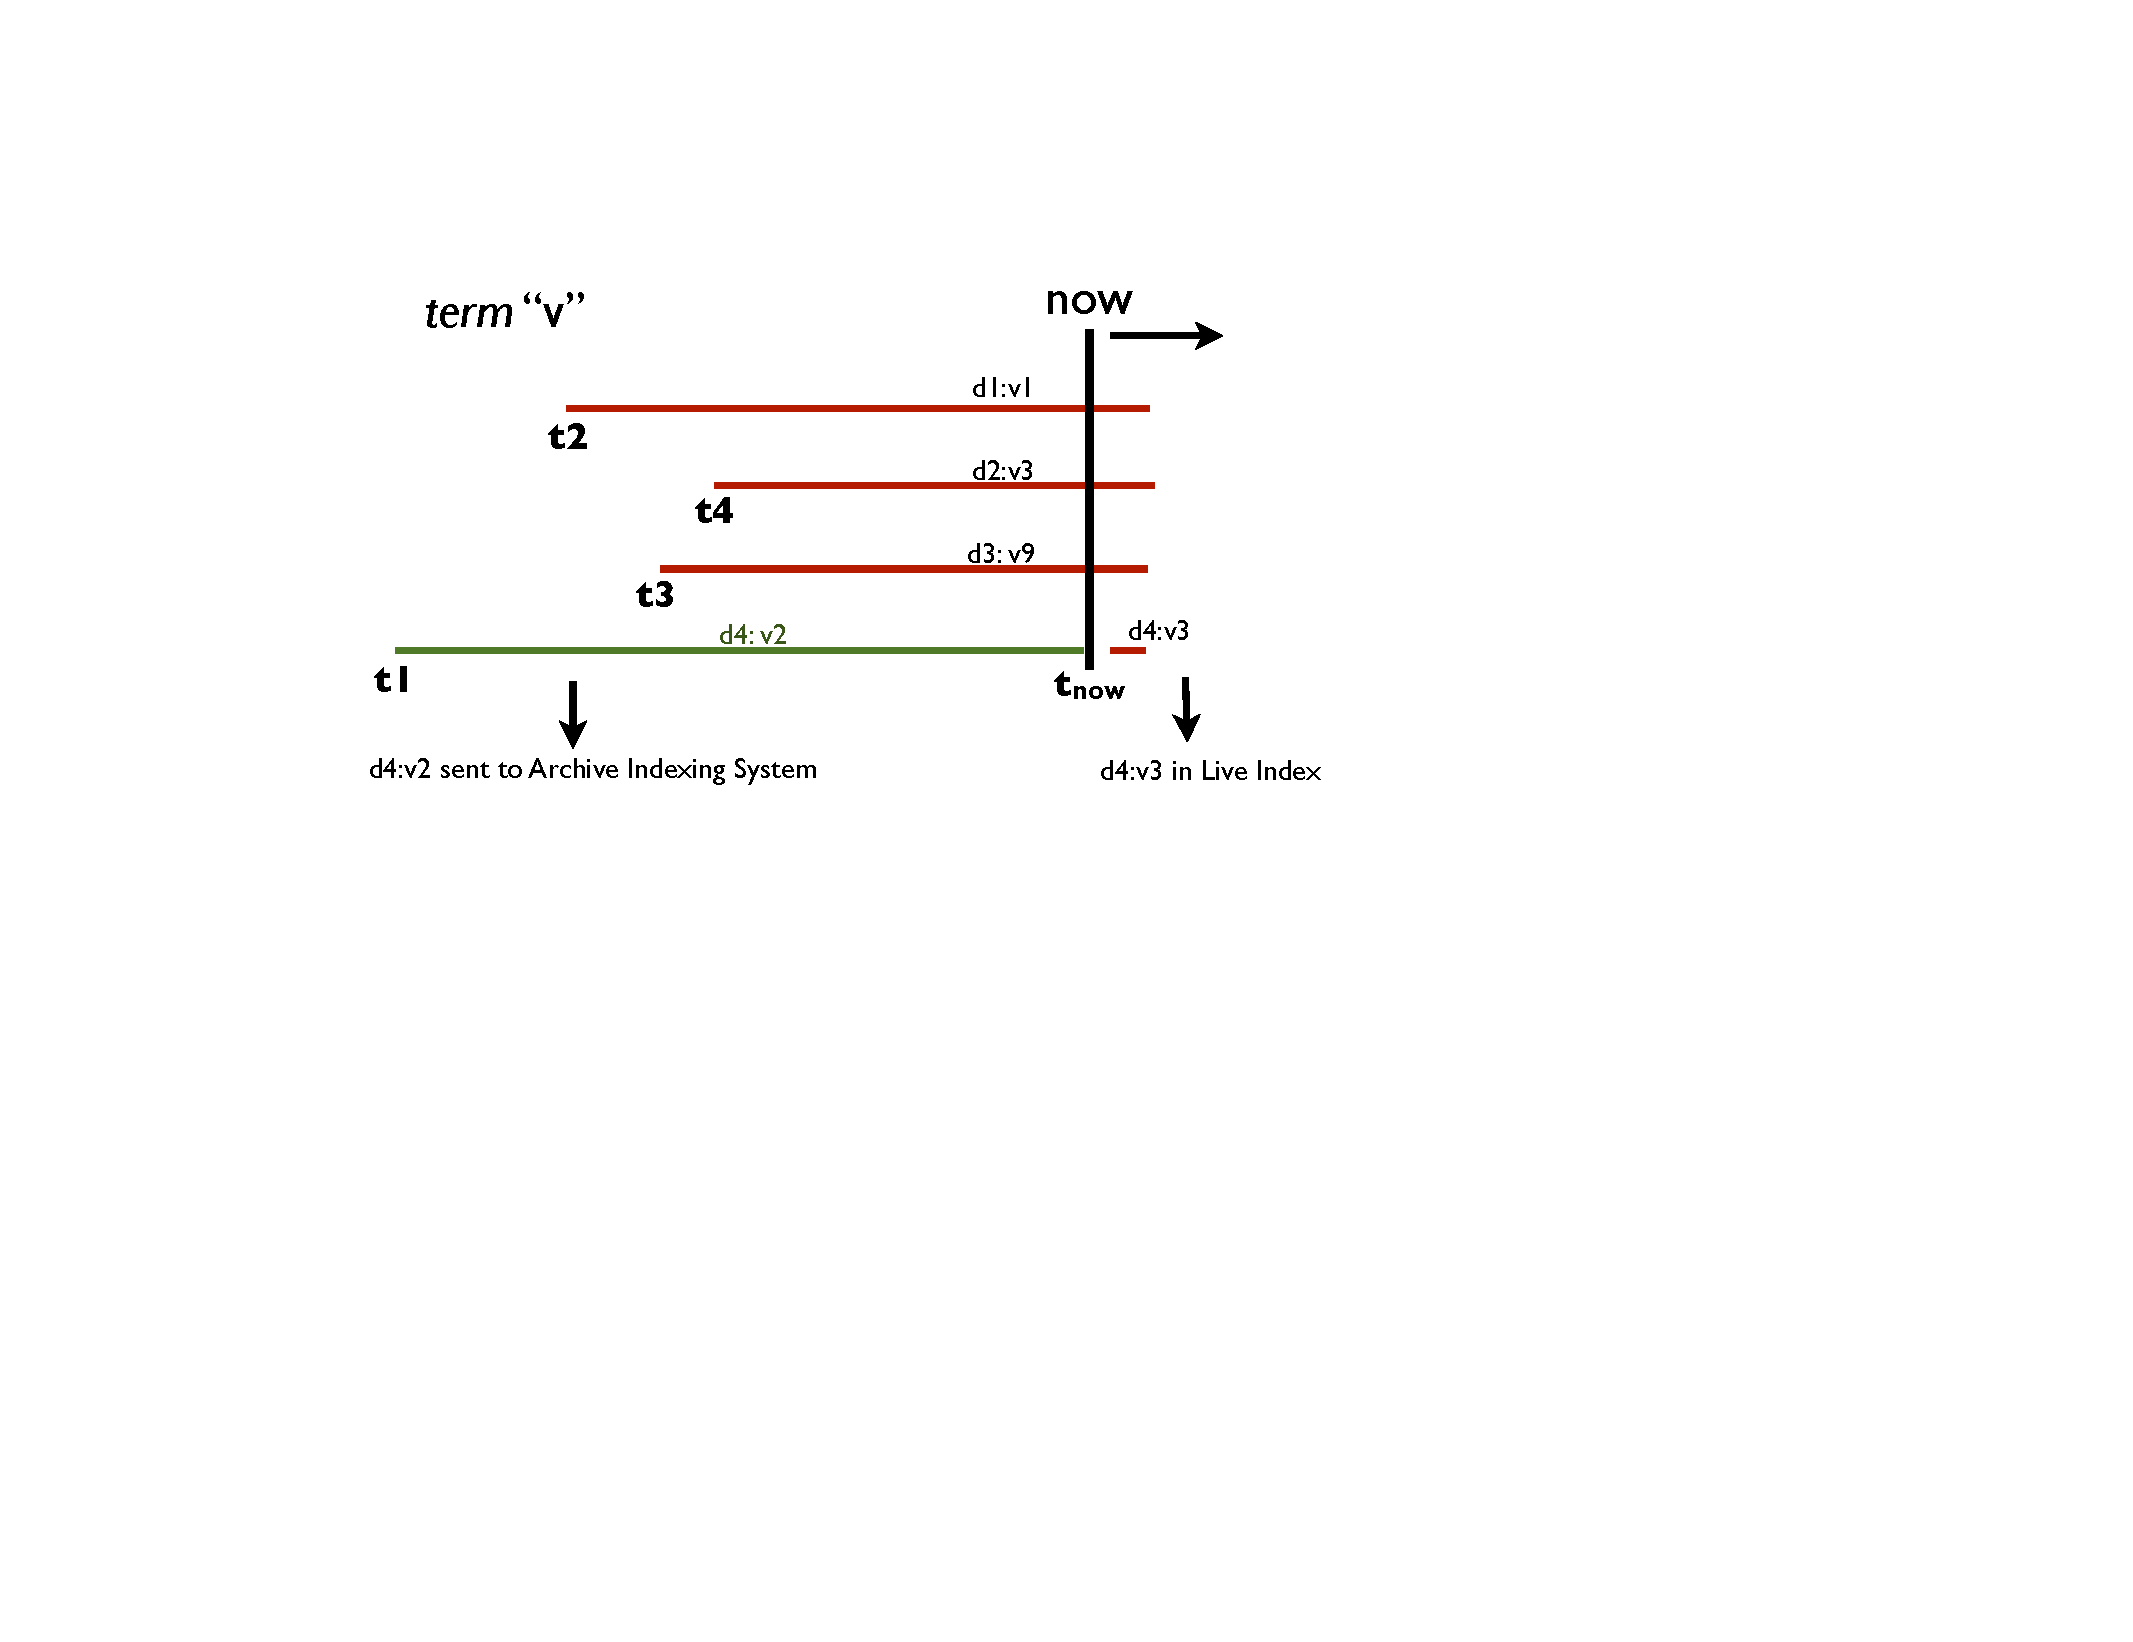
\includegraphics[width=0.475\textwidth]{resources/sliding_wind.pdf}
	\caption{End time order of finalizing versions}
	 \label{fig:finalizing_versions}
\end{figure}

\begin{figure}[tb]
	\centering
		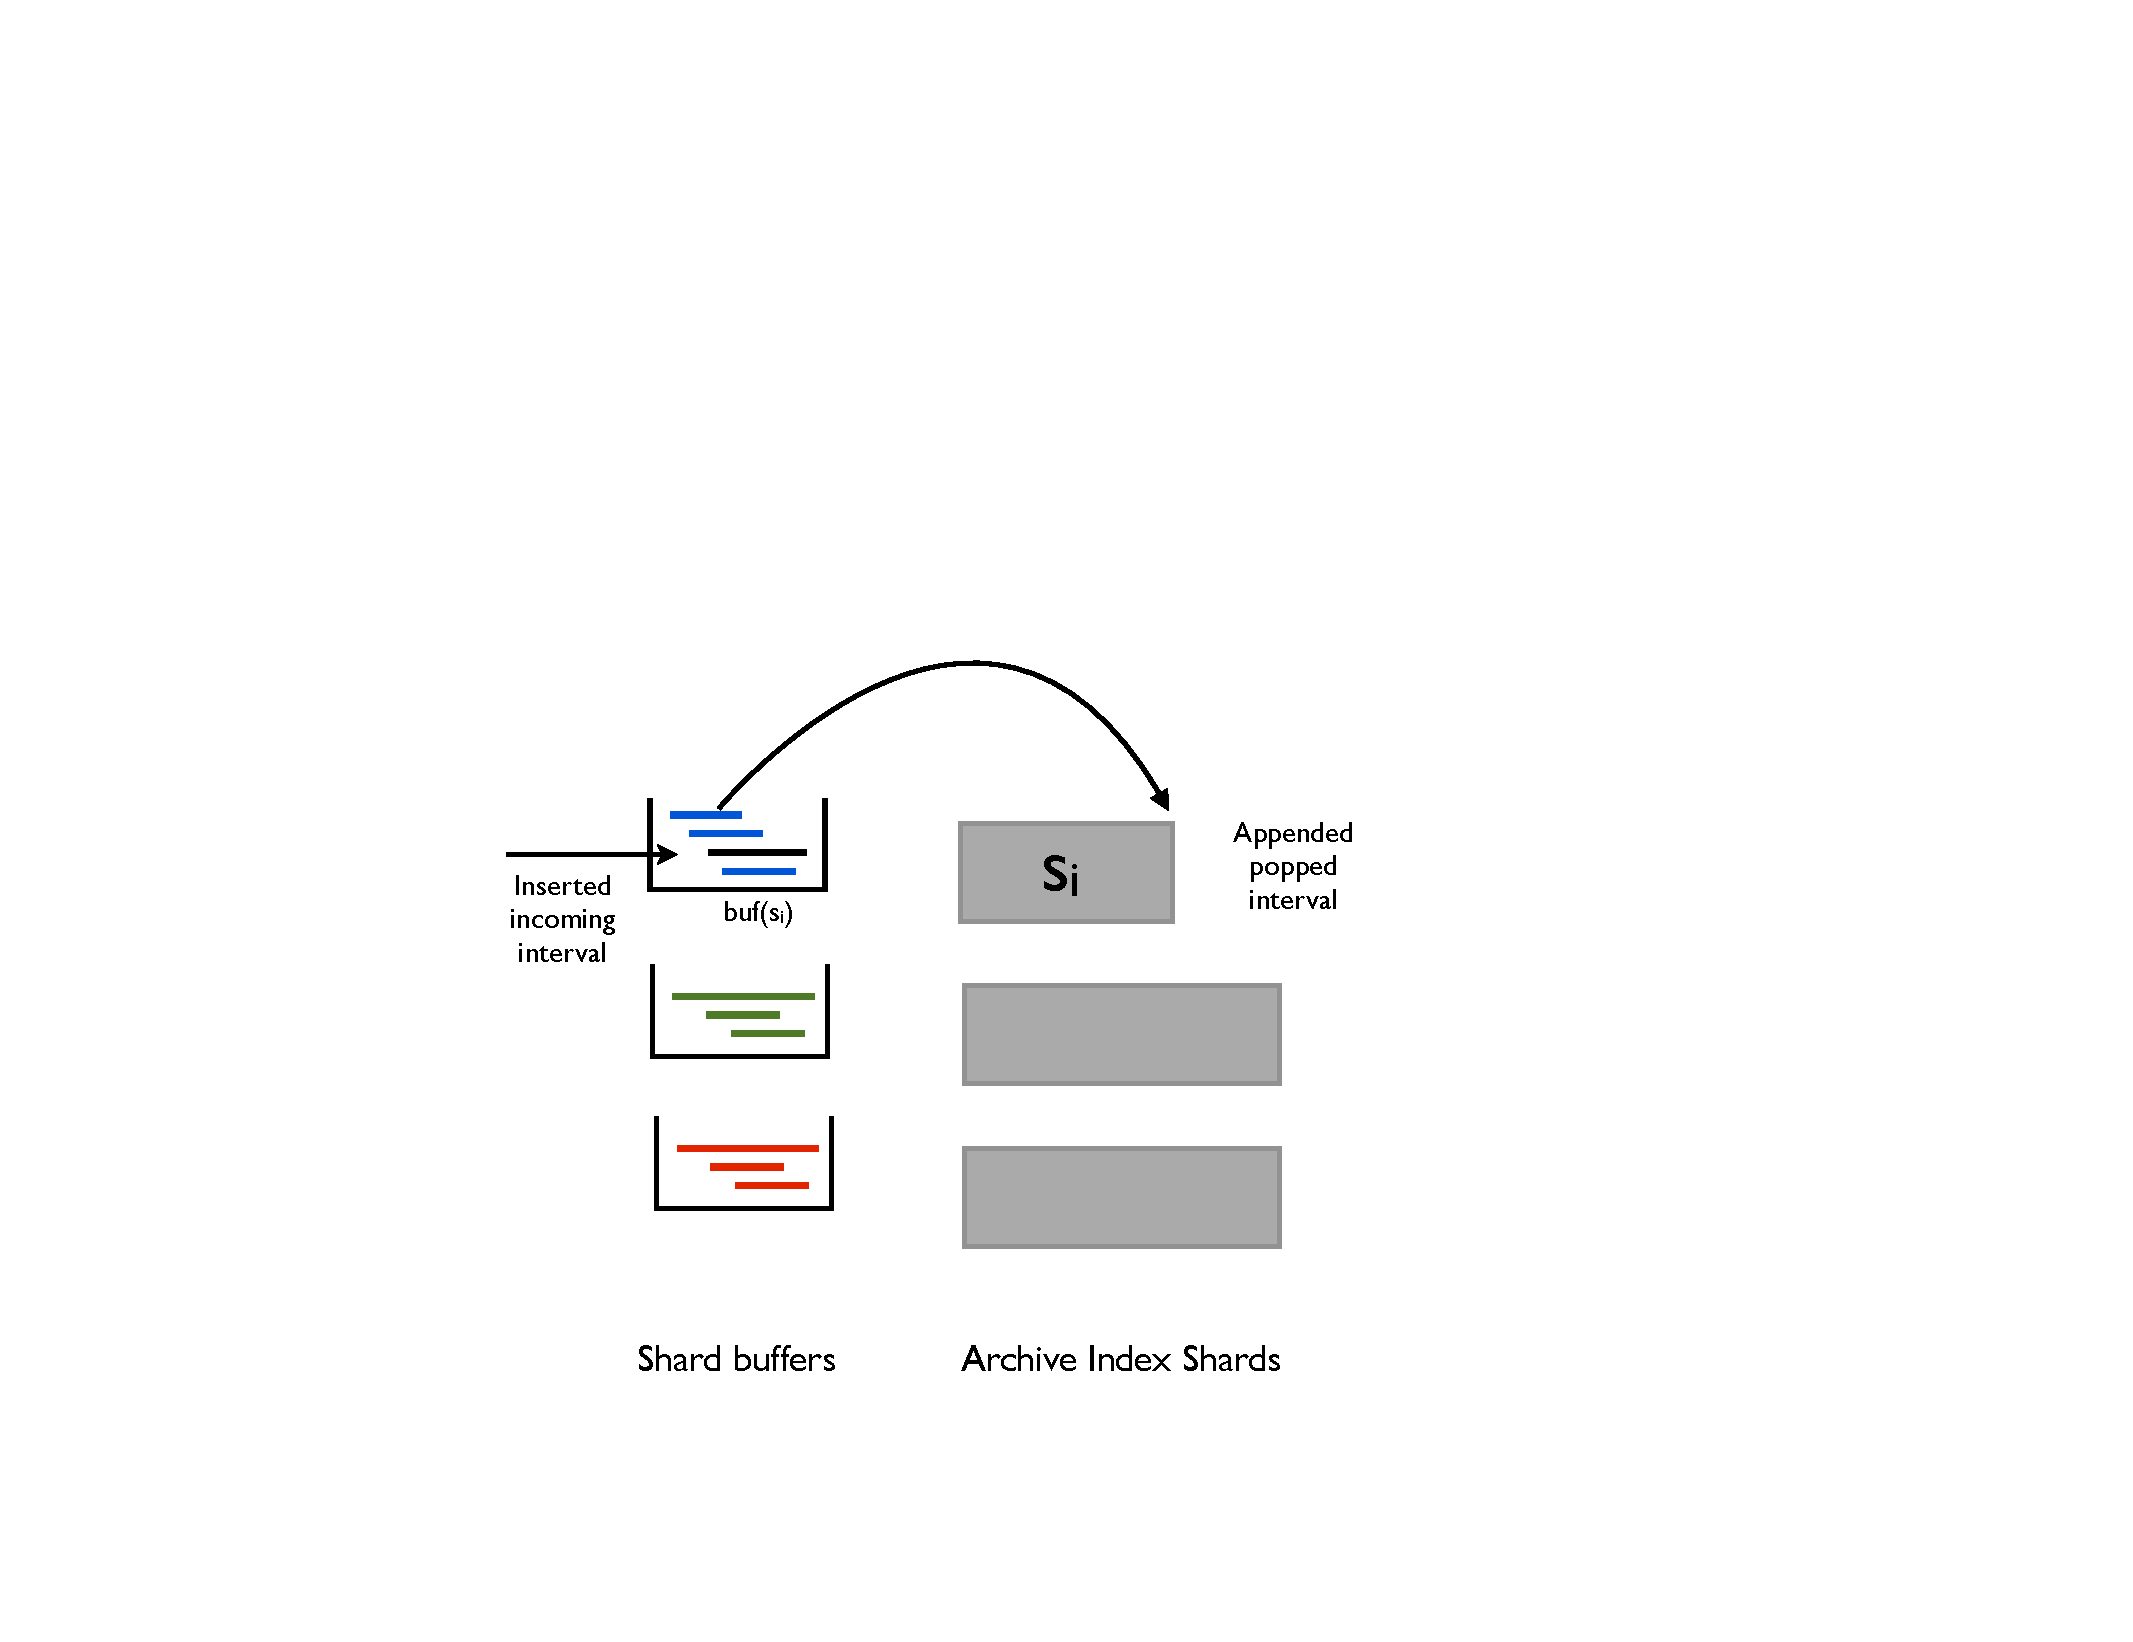
\includegraphics[width=0.475\textwidth]{resources/inc_sharding.pdf}
	\caption{Incremental sharding}
	 \label{fig:inc_sharding}
\end{figure}


\begin{definition}[Bounded Subsumption]
A shard $S$ is said to satisfy the bounded subsumption property of limit $\eta$ if each interval $I_i \in S$ does not subsume more than $\eta $ intervals:
$$ \forall I_i \in S: \vert \,\{ \, I_j \in S \, \mid \, I_j \neq I_i \,\, \wedge \,\, I_i \sqsupset I_j \} \,\vert \,\leq \, \eta  \,\,.
$$\end{definition}

The problem of minimizing the number of random accesses with a limited number of wasted sequential accesses can be redefined in terms of minimizing the overall number of shards such that each shard exhibits the bounded subsumption. Thus, the problem definition becomes:
%Since we intend to minimize the number of random accesses given a bound on the wasted sequential accesses we want to minimize the number of shards, a problem which can be formally defined as follows:%We define the problem of minimizing the overall number of shards such that each of them exhibits the bounded subsumption property as the following:

\begin{definition}
Given a set of intervals $\mathcal{I}$, partition $\mathcal{I}$ into a \emph{minimal set} of shards  $\mathcal{S} = \{S_1, \ldots, S_{m}\}, \, \forall I_k \in S_{i}, \,\, I_k \in \mathcal{I}$ where:
\begin{eqnarray*}
	S_i \cap S_j = \emptyset & \forall S_i, S_j \in \mathcal{S}, \; i \neq j \\
	\bigcup_{i}{S_i} =  \mathcal{I} & \\
	\mathrm{s.t.}\quad \forall S_i \in \mathcal{S} &:\,S_i \mathrm{~satisfies~bounded~subsumption}.
\end{eqnarray*}
%\hfill $\Box$ 
\end{definition}

Before attempting to solve the above problem let us discuss certain properties in an archive indexing setting. Firstly, the archive setting is very specific in terms of arrival of the input sequence, i.e., in the order of arrival of new versions to the archive index. Whenever the end time of an existing version is determined, it is sent to the archive indexing system (refer Figure~\ref{fig:finalizing_versions}). Since versions are generated in the end time order, the input intervals also follow the same order. 

Secondly, we do not deal with deletions of versions since a deletion of a document results in an entry in the archive index for that document, and existing versions are never removed. This means that the index steadily grows over time with the older collection indexed by the archive index being a subset of the current collection. 

Finally, from the indexing point of view it is preferable to have an updating scheme which appends newly created postings at the end of the index list. The major benefit of an append operation is that the indexes built for the older indexes can be used as partial solutions to build an up-to-date archive index efficiently thus avoiding recomputation. Recomputation of shards with a non-append based technique (say cost-aware sharding) is expensive because it involves processing the entire input (existing data along with the new updates) thus limiting its applicability to an update aware indexing system. 

Another benefit with an append operation is the avoidance of the expensive decompression and compression cycles in building the new updated index. While merging two index lists by employing recomputation the corresponding shards of each term are completely decompressed to form usable input for the sharding algorithm. After recomputing the new set of shards are compressed back again for storage. The most popular compression algorithms used in index list compression are based on gap-encoding schemes which are local schemes and hence append friendly. Hence, rather than optimally solving the problem we look for an approach which is based on an append only operation to the existing shards and exploits the end time order of input arrival. In the following subsection we introduce the \emph{incremental sharding} algorithm which apart from being incremental also has an approximation guarantee. 

%Another benefit of sharding incrementally is that the indexes built for the older indexes can be used as partial solutions to build an up-to-date archive index thus avoiding recomputation. 
\subsection{Incremental Sharding Algorithm}

We present the \emph{incremental sharding algorithm} which is an update aware incremental algorithm with a factor $(2  -  \frac{2}{\eta+2})$ approximation algorithm(cf. Algorithm~\ref{alg:rs-inc}). Apart from having the natural benefit of being an append only algorithm it also exploits the end time arrival order of the intervals %(c.fSection~\ref{fig:finalizing_versions}) 
by processing the intervals in that order thus avoiding expensive sort operations on the input. 

 % The reason for such an algorithm is firstly because it adds intervals to the existing shards in an append-only style which is essential for index updates. We will see later that an optimal solution to relaxed sharding might result in inserts in the beginning of the lists, which makes updates particularly expensive. Secondly, it processes the intervals in end time order which is the natural sequence of arrival of new versions or finalization of the old versions. 

The algorithm processes intervals in the end time order (cf. line 1) and creates or updates shards incrementally. It follows a scheme of immediate assignment but deferred append of an interval to a shard. For each shard we maintain a \emph{shard buffer} of size $\eta+1$ and an \emph{shard begin time}. The assignment of the interval to a shard is based on the begin time of the shard and the shard buffer defers the actual writing or appending of the interval of the shard to satisfy the bounded subsumption property. In other words the shard buffer maintains the interval until it deems it right to be appended to the end of the shard.

When an interval, $I[i]$, is processed it is either assigned to an existing shard based on the interval and shard begin times (cf. line 15) or it results in the creation of a new shard (lines 7-10). The creation of a new shard involves setting the begin time of the shard to zero and placing the chosen interval in its shard buffer. Until the buffer reaches its capacity of $\eta$ the begin time of the shard remains zero. The shard begin time is first updated only when the an interval is popped out of it after the buffer reaches its capacity $\eta+1$.  When the assignment for the interval is decided, say $S_t$, it is placed in the respective shard buffer $bu\!f(S_t)$ (cf. line 19). The incremental sharding chooses the shard whose begin time has the least difference with the begin time of the incoming interval (cf. line 15). 

The shard buffers determine the relative position of the intervals in the shard where it will be finally stored. The insertions into the buffer are made to preserve the begin time order (cf. line 19) which in turn ensures a begin time order when intervals are removed from it. This is diagramatically shown in Figure~\ref{fig:inc_sharding}. Only the first interval or the interval with the minimum begin time is removed from the buffer to limit the buffer size to $\eta + 1$ (line 23) and it is appended to the end of its corresponding shard $S_t$. The shard buffers also ensure that no interval in a shard subsumes more than $\eta$ intervals. This is done by setting the begin time of a shard $S_t.begin$ to the first interval $begin(first(bu\!f(S_t)))$(or the interval with the least begin time) of the shard buffer as in line 24. The interval with the minimum begin time in the shard can subsume the maximum number of intervals and any interval with a begin time lesser than it is dissallowed.

Note the use $\cup$ in lines 23 and 30 to indicate the \emph{append} operation on the shard that is logically organized as a list of intervals in their begin time order.


% Observe that  operator $\cup$ used might be misleading in lines 23 and 30. We intend an append operation to the shard that is logically organized as a list of intervals in their begin time order.

 \begin{algorithm}[htb]
   %\small
   \begin{algorithmic}[1]
     \STATE  \emph{Input:} (i)$\eta$, (ii)$\mathcal{I}$ sorted in increasing order of end times
     \STATE $\mathcal{S} = \emptyset$ \quad // incremental sharding
 		
	\STATE \FOR{$i = 1\,..\,|\mathcal{I}|$} 
	\STATE //creates new shard
        \IF {$\neg \exists S \in \mathcal{S} : S.begin \, \leq \, begin(I[i])$} 
        		\STATE create \textbf{new shard} $S_{new}$ and $bu\!f(S_{new})$ \\
			%\STATE $g_{new}.begin = begin(I[i])$ 
			%\IF {$\eta > 0$} 
				\STATE $S_{new}.begin = 0$
			%\ENDIF
			
			\STATE \textbf{add} $I[i]$ to $bu\!f(S_{new})$  
                     \STATE $S = \mathcal{S} \cup \{S_{new}\}$
        \ENDIF

	\STATE 

			\STATE //find the best candidate shard for assignment
			\STATE $S_{cand} = \{ S_i \,\,|\,\, S_i \in \mathcal{S} \,\, \wedge  \,\,S_i.begin \leq begin(I[i])\}$
			\STATE $S_{t} =\argmin{g\, \in \,S_{cand}} (begin(I[i]) - g.begin)$ 

		\STATE
		\STATE //update buffers and begin times of shards
		\IF { $S_t \neq S_{new}$}
			\STATE \textbf{insert} $I[i]$ into $bu\!f(S_{t})$ in begin time order			 
		\ENDIF
		\IF {$|bu\!f(S_{t})| = \eta+1$}
			\STATE  //first element in the buffer finalized
			\STATE $S_{t}$ = $S_{t} \,\, \cup$  $removefirst(bu\!f(S_{t}))$
			\STATE  $S_{t}.begin$ = $begin(first (bu\!f(S_t)))$
		\ENDIF        
   	\ENDFOR 
	\STATE
	\STATE //finally append the buffer intervals to the shards
	\FOR {$S \in \mathcal{S}$}
		\STATE	$S \,\,= \,\, S \,\cup bu\!f(S)$
	\ENDFOR
\STATE
\STATE\emph{Output:} $\mathcal{S}$  is the incremental sharding.

   \end{algorithmic}
   \caption{Incremental Sharding Algorithm}
   \label{alg:rs-inc}
 \end{algorithm}


\subsection{Approximation Guarantee}
\label{proof:approx_guarantee}

\begin{theorem}
\label{thm:inc_sharding}  
Incremental sharding is a $(2- \frac{2}{\eta+2})$ approximation.
\end{theorem}

We approach the proof by first proving two lemmas.
Assuming that incremental sharding produces $m$ shards, we construct a worst case scenario. For notational convenience let us assume that shards are numbered according to their creation times in incremental sharding, i.e., $S_1$ was created before $S_2$ and so on. 

\begin{lemma}[Descending Begin Times]
\label{lem:descending_begintimes}
If incremental sharding created a shard $S_{i+1}$ after $S_i$, then \linebreak $S_i.begin > S_{i+1}.begin$.
\end{lemma}
\begin{proof}
We prove this property by induction over increasing number of intervals $I_i \in \mathcal{I}$ which are added in in end time order, i.e, $end(I_{i+1}) \, > \, end(I_{i})$ .

$i = 1:$ For the first interval $I_1$ the property holds since there are no earlier shards.

$i \rightarrow i+1$: Let there be $n$ existing shards $\mathcal{S} = \{ S_1 \cdots S_n \}$. Depending on the begin time of the $(i+1)$th interval $begin(I_{i+1})$ we consider the following two cases:

\emph{Case 1:} If $begin(I_{i+1}) < S_k.begin \,\, , \,\, 1 \le k \le n$, then $I_{i+1}$ forms a new shard $S_{new}$ and the begin of the shard $S_{new}.begin$ is less than all the existing shard begin times. This proves the claim.

\emph{Case 2:} Assuming $\exists S_k : begin(I_{i+1}) \geq S_k.begin$ and on addition of $I_{i+1}$ to $S_k$ there is a violation of the descending begin time order of shards, i.e. , $S_k.begin > S_{k-1}.begin$. This means that $S_{k-1}.begin < begin(I_{i+1})$ and $I_{i+1}$ should have been assigned to $S_{k-1}$ due to a smaller difference according to the induction hypothesis of $S_{k+1}.begin > S_{k}.begin\,\,, \,\,\forall 1 \le k < n$.
\end{proof}

\begin{lemma}[Incremental subsumption]
\label{lem:incremental_subsumption}
	An interval \linebreak added to $S_i$ subsumes at least $(i-1)(\eta + 1)$ intervals.
\end{lemma}


\begin{proof}
Note that $S_i.begin$ refers to the time of the first interval in the buffer of shard $S_i$ or the earliest begin time in the shard buffer $bu\!f(S)$. 
By Lemma~\ref{lem:descending_begintimes} we know that there is an ordering of the shard begin times. Hence for an interval $I$ assigned to $S_i$ the following holds -- $begin(I) < S_{i-1}.begin < \cdots < S_1.begin$. Since we assume end time arrival order of intervals it subsumes all intervals in $i-1$ shards buffers, which are $S_1,...,S_{i-1}$. Further the fixed buffer size of $\eta+1$ results in making the subsumptions lower bounded by  $(i-1)(\eta + 1)$.\end{proof}

We recollect the \emph{Staircase Property} of a shard as introduced in~\cite{aanand:sigir2011} as a property which requires the intervals to be in their begin time order and additionally disallowing subsumptions among any pair of intervals in the shard. We further need to introduce the notion of \emph{stalagtite sets} and \emph{stalagtite groups}. A \emph{stalagtite set} $\Lambda_s$ is a set of time intervals such that,
$$\forall p, q \in \Lambda_s, begin(p) \leq begin(q) \Rightarrow end(p) > end (q) .$$

\emph{Stalagtite groups} (cf. Figure~\ref{fig:stalagtite_groups}) are a collection of sets of intervals such that choosing one interval from each of these sets results in a \emph{stalagtite set}. 

\begin{lemma}[Stalagtite grouping]
\label{lemma:stalagtite_grouping}
Stalagtite grouping with a staircase property in each shard is the worst case for incremental sharding.
\end{lemma}
\begin{proof}
From the previous lemma, any input resulting in $m$ shards from incremental sharding will have at least intervals with $\eta+1$, $2(\eta+1)$, $\cdots$, $(m-1)(\eta+1)$ subsumptions in $S_2, S_3, \cdots, S_m$ respectively. Let us suppose that the set of subsumed intervals when the first interval added to $S_i$ be represented as $sub(S_i)$. To reduce the overall number of shards we should strive for a configuration with minimum number of subsumptions. This is possible when $sub(S_1) \subseteq sub(S_2) \subseteq \cdots \subseteq sub(S_m)$ and $|S_i| = \eta + 1, \forall i = 1,\ldots,m$. This arrangement forms a \emph{stalagtite group}(cf. Figure~\ref{fig:stalagtite_groups}) with each of the groups having a cardinality of $\eta+1$.


Additionally, each of these stalagtite groups should have a staircase arrangement to allow for the maximum capacity - $\eta$ - out of place insertions. Any additional interval or misaligned interval either increases subsumption or reduces capacity for out of place insertions. Any removal of intervals on the other hand result in contradiction to the original assumption that there are $m$ shards from incremental sharding.
\end{proof}


\begin{figure}[tb]
  	\centering
		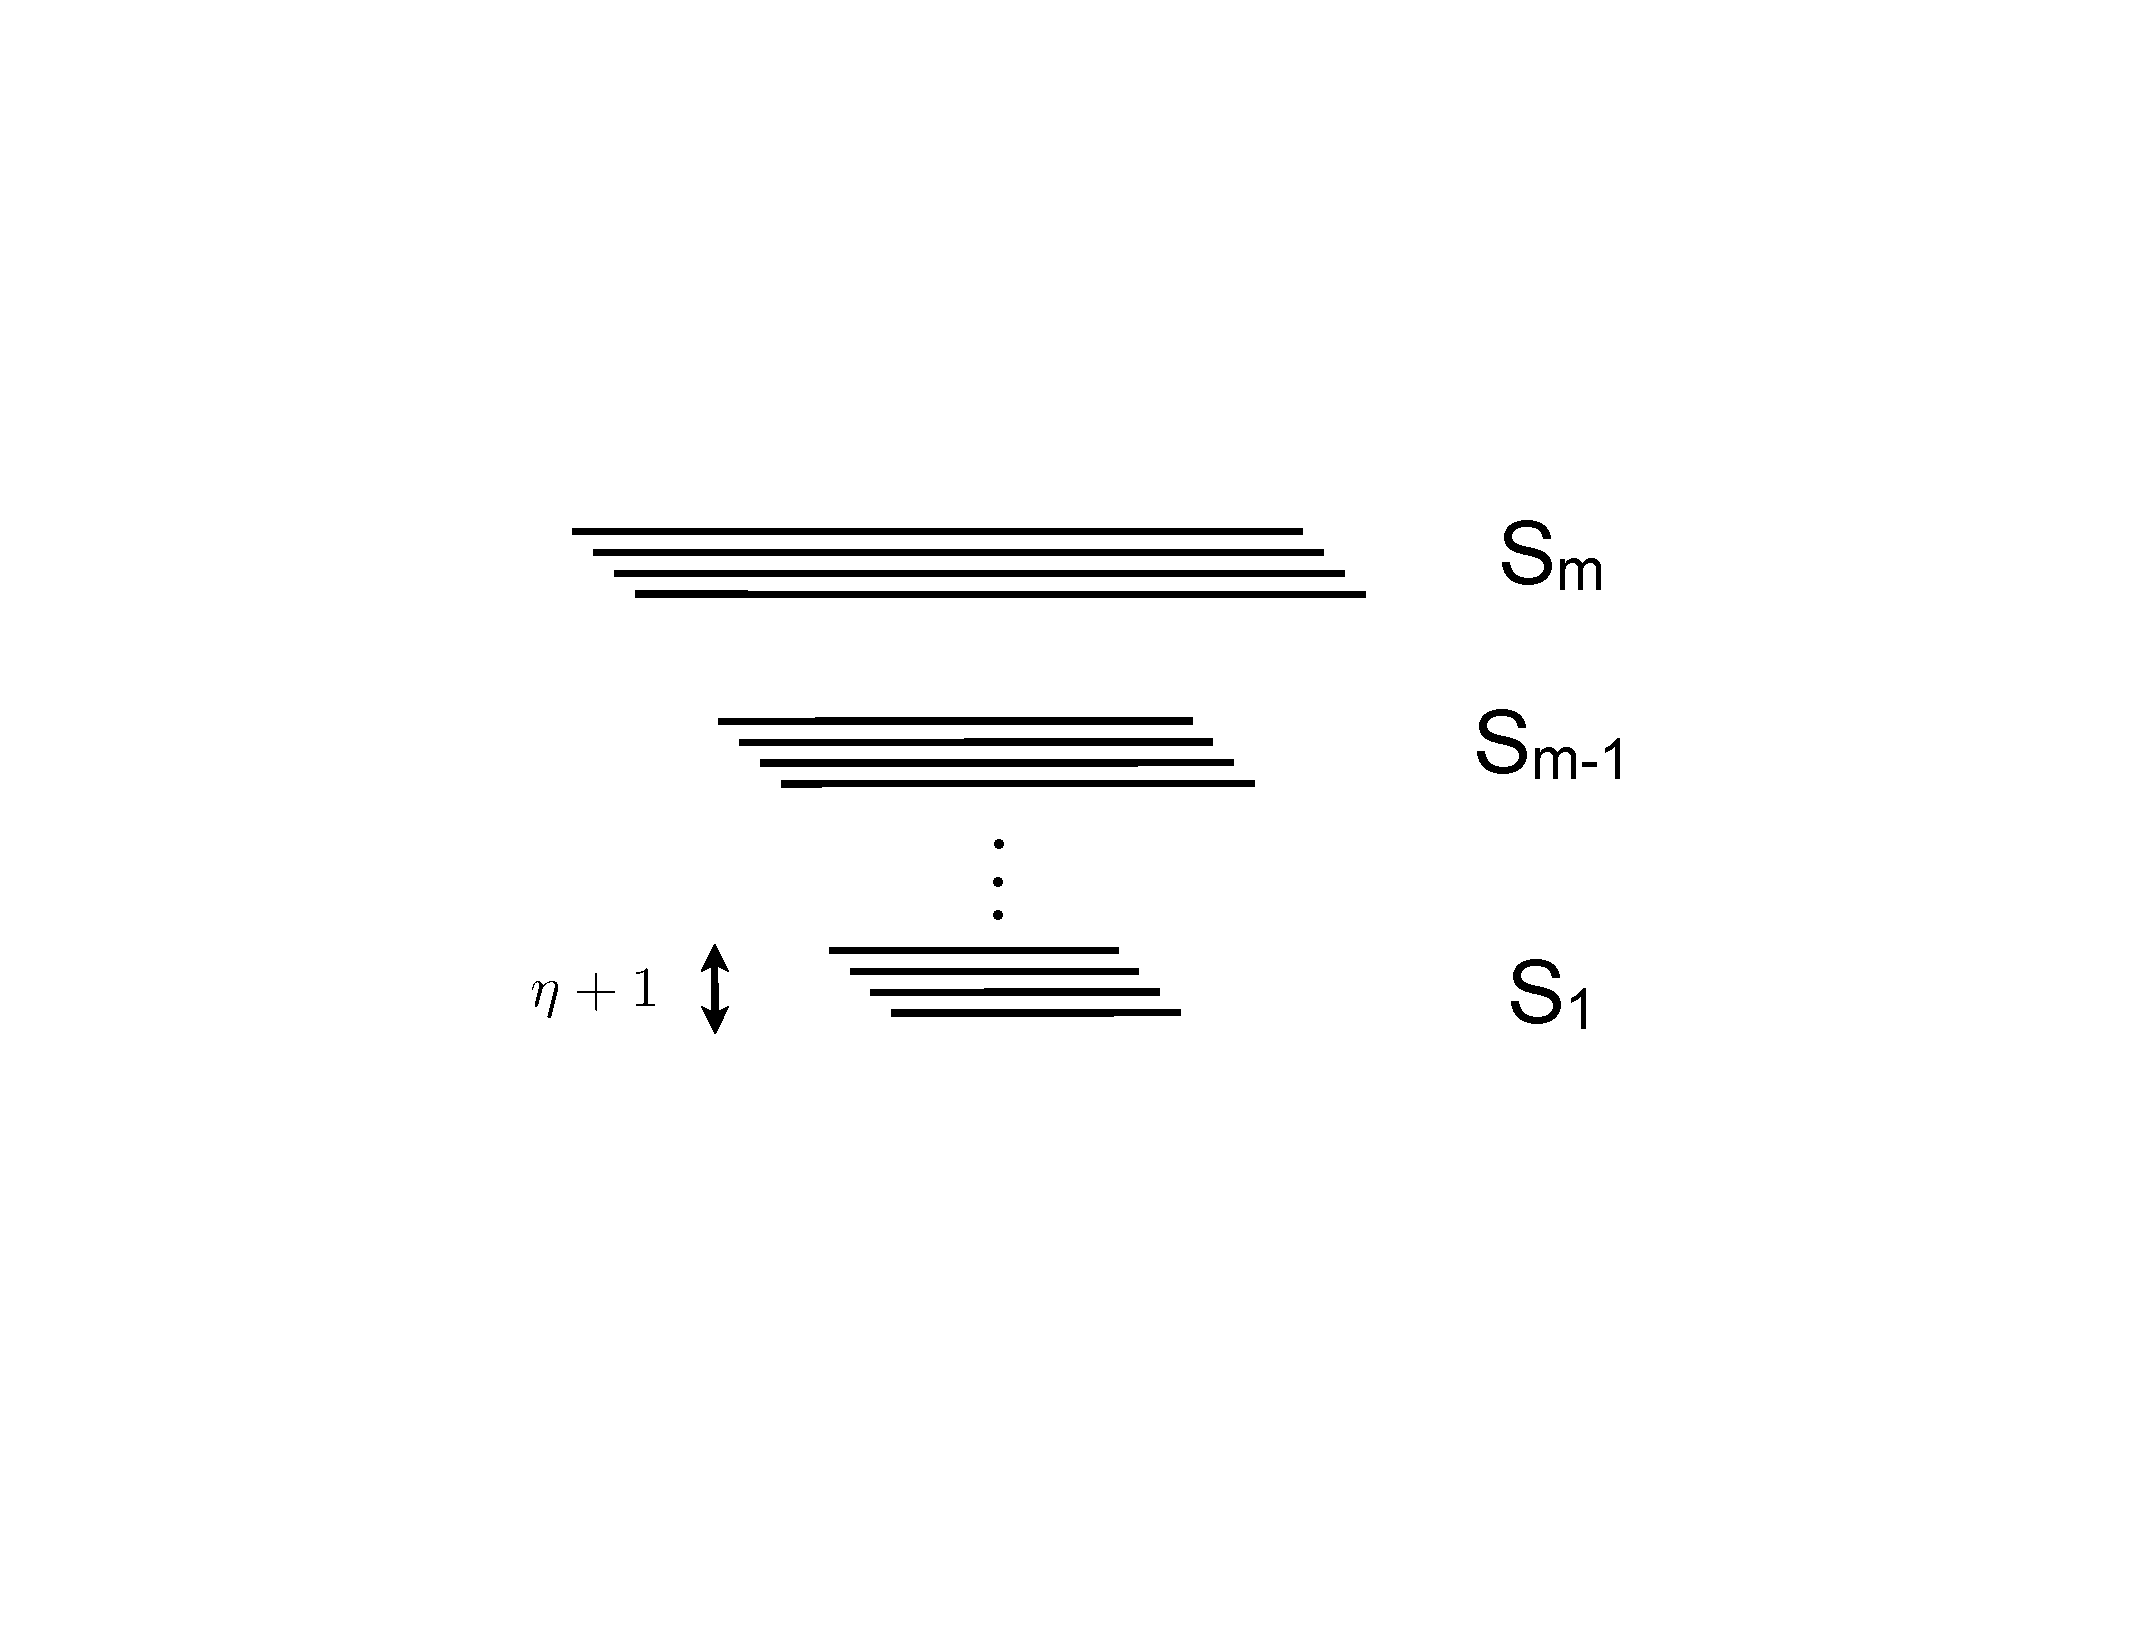
\includegraphics[width=0.375\textwidth]{resources/stalagtite_grp.pdf}
   	\caption{Stalagtite groups}
		  \label{fig:stalagtite_groups}	
\end{figure} 

Now we can complete the proof for Theorem 1.%~\ref{thm:inc_sharding}.
\begin{proof}
From the Lemma~\ref{lemma:stalagtite_grouping} we know that there are $m$ stalagtite groups with each group residing in the shards formed from incremental sharding. It is easy to see that none of the optimal shards will have more than $2\eta + 1$ intervals. Thus we choose an assignment where we try to minimize minimum number of shards, i.e., choose as many shards with $2\eta + 1$ intervals as possible. One such assignment is when we assign $\eta$ of the $\eta+1$ intervals of $S_i$ to $S_{m+1-i}, \,\, \forall i \leq \frac{m}{2}$. The remaining $\frac{m}{2}$ intervals (an interval from each $S_i$) can then be placed in $\frac{m}{2(\eta+1)}$ shards. Hence for $m$ shards created by incremental sharding  we get a minimum of $\frac{m}{2} + \frac{m}{2(\eta+1)}$ shards. Notice that we can have other arrangements which give the same number of minimum shards. The ratio 

$$
	\frac{|S|}{OPT} = \frac{m}{\frac{m}{2} + \frac{m}{2(\eta+1)}} 
					= 2 \left(1 - \frac{1}{\eta + 2}\right)
$$

proves that incremental sharding is a factor $(2  -  \frac{2}{\eta+2})$ approximation algorithm.
\end{proof}

% System Architecture

%!TEX root = ./sigir2011.tex
\section{System Architecture}
\label{sec:system}

\begin{figure}[tb]
  	\centering
	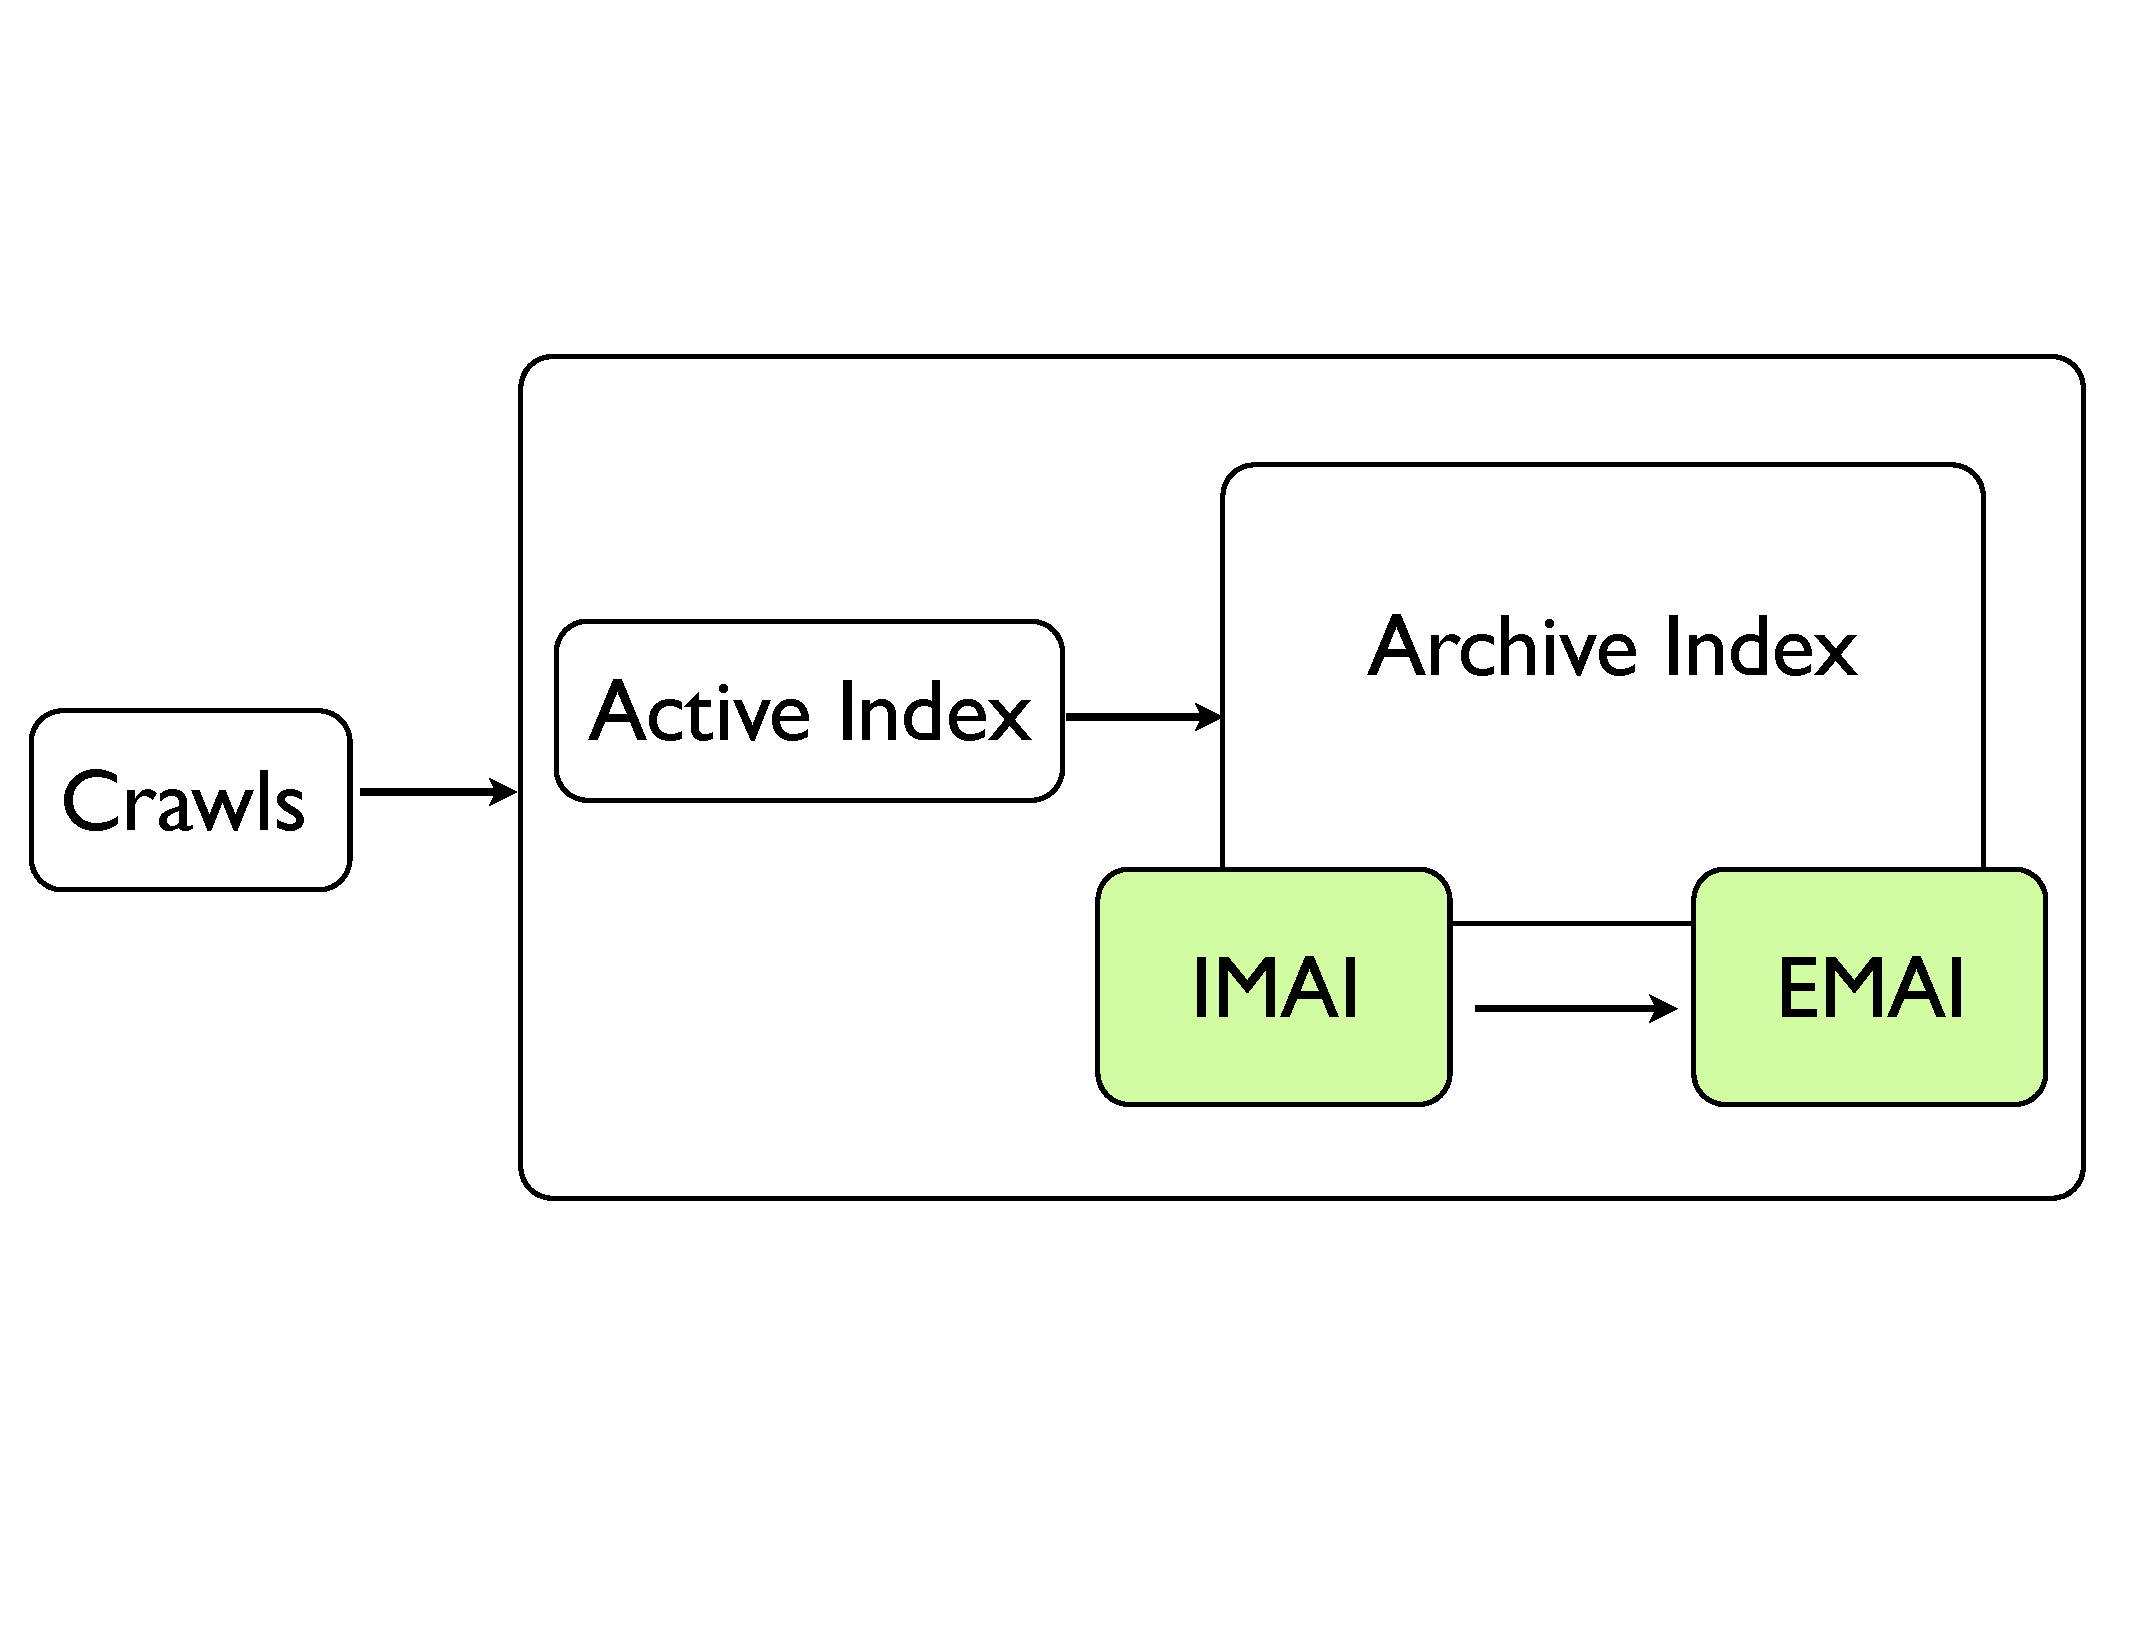
\includegraphics[width=0.5\textwidth]{resources/system_arch_incsh.pdf}
   	\caption{System architecture}
		  \label{fig:archive_indexing_system}	
\end{figure}

Figure~\ref{fig:archive_indexing_system} shows a high-level overview
of the architecture of a search engine using our incremental sharding
method. It consists of
\begin{itemize}
\item The \emph{active index} for all active versions of documents,
  consisting of an in-memory inverted list for each term that keeps
  the active versions of documents containing this.
\item The \emph{archive index} for all archive versions of documents,
  consisting of an inverted list for each term that is organized in
  shards. The archive index consists of an in-memory index \emph{IMAI}
  and an on-disk index \emph{EMAI}, both organized in shards.
\item A \emph{crawler} that continuously crawls the target Web sites,
  for example a predefined set of domains or the complete Web.
\end{itemize}

When the crawler encounters a new document that has been unknown so
far, it adds it to the active index; this is an inexpensive operation
since the active index is in main memory. When a document is found
again, it is checked for changes (using, for example, a fingerprinting
technique such
as~\cite{DBLP:journals/cn/BroderGMZ97,DBLP:conf/sigir/Henzinger06}). If
changes are detected, the active version of that document turns into
an archive version (with end time equal to the crawl time) and is
sent to the archive index, and index entries for the new active
version are added to the active index.

The archived version is then added to the in-memory archive index by
first creating the corresponding postings for each term, which are
then added to the in-memory archive index using the incremental
technique from
Section~\ref{sec:inc_sharding}. Figure~\ref{fig:finalizing_versions}
shows an example for this, where in a crawl at time $t_{now}$ a new
version $v_3$ for document $d4$ is detected. This results in firstly
adding a new version $d4:v3$ with a begin time $t_{now}$ to the
affected terms in the active index. Secondly, the end time of $v2$ is
finalized and the posting $\langle d4:v2, [t_1, t_{now}], \, score
\,\rangle$ with the complete interval information is send to the
archive indexing system. In the archive indexing system this posting
is processed by placing it in the shard buffer of term ``v" and
updating the IMAI from the popped posting in the buffer as shown in
Figure~\ref{fig:inc_sharding}.  As soon as the in-memory index IMAI is
full, entries are merged into the disk-based archive index EMAI,
merging corresponding shards; this essentially corresponds to
incremental maintenance of standard inverted lists.

% Experimental Evaluation

\section{Experimental Evaluation}
\label{sec:eval}
\begin{table*}
  \center
  \begin{tabular}{l c c r r r} 
      \toprule
      { Dataset} & \multicolumn{1}{c}{Coverage}&  \multicolumn{1}{c}{Size (in GB)} & \multicolumn{1}{c}{$\mathcal{N}$} & \multicolumn{1}{c}{$\mathcal{V}$} & \multicolumn{1}{c}{$\mu / \sigma$}\\
      \midrule
      {\bf WIKI} & 2001  to 2005  & $\sim$700 & 1,517,524 & 15,079,829 & 9.94 / 46.08\\

      {\bf UKGOV} & 2004 to 2005 & $\sim$400 & 685,678 & 17,297,548 & 25.23 / 28.38\\
      \bottomrule
    \end{tabular}\\
    \hspace*{2ex}\parbox{0.65\textwidth}{\fontsize{8pt}{8pt}\sffamily Datasets with no. of documents $\mathcal{N}$,
    no. of versions $\mathcal{V}$, average number of versions per documents~${\mu}$, and standard deviation~${\sigma}$.}
  \caption{Characteristics of datasets used}
  \label{tab:datasets}
\end{table*}

% Setup:
% ====

%1) Hardware setup:
%	as in earlier works
%2) Dataset description: 
%	as in earlier works
%3) Index Construction : 
%	 a) Partial Indexes with monthly granularity
%	 b) index versions which end exactly in the month
%	 c) Compression = 7 bit + coalescing
%4) Query workload:
%	warm cache experiments (5 runs with avg of 4). week, monthly and year duration queries. 330 popular queries from the AOL querylog. for each we randomly generate 3 week, month, year duration queries. 
%5) For merging we employ immediate merge to make one single index. <refs from buttchers paper> Other techinques are complementary.

%6) Stats from Index sharding:
%	Avg. number of shards for CAS and Incsh for different param. values
%	Size of the monthly partitions
%	Clarify the point that other approaches are complementary since the merging of 2 larger size partitions have high time anyways




%\subsection {Experimental Setup and Datasets}
All our algorithms were implemented in Java 1.6, within the
time-travel indexing system presented earlier in
~\cite{aanand:sigir2011}.  Experiments were conducted on Dell
PowerEdge M610 servers, with 48 GB of main memory, and attached to a
large disk array through iSCSI.

% Our implementation was based on the Java-based code we earlier
% in~\cite{aanand:sigir2011}

% In order to ensure consistency of experimental setup, we retained
% the hardware specificationsused in the

% All experiments were conducted on Dell PowerEdge M610 servers with 2
% Intel Xeon E5530 CPUs, 48 GB of main memory, a large iSCSI-attached
% disk array, and Debian GNU/Linux (SMP Kernel 2.6.29.3.1) as
% operating system. Experiments were conducted using the Java Hotspot
% 64-Bit Server VM (build 11.2-b01).

% We implemented our algorithms using Java 1.6. Additionally, we
% obtained the latest implementation of sharded indexes from the
% authors of~\cite{aanand:sigir2011}.

% \subsection{Datasets}
The two data collections used in our experiments are: (i) the English
Wikipedia revision history, referred to as the {\bf WIKI} collection,
which contains the edit history from January~2001 until December~2005
excluding all the minor edits, and (ii) a web archive, referred to as
the {\bf UKGOV} collection, provided by the Internet Memory Foundation
(previously European Archive), consisting of weekly crawls
of 11 government websites within U.K. during 2004 and 2005. The
characteristics of these two collections are briefly summarized in
Table~\ref{tab:datasets}. For the ease of experimentation, we rounded
the time-stamps of versions to the nearest day for all datasets.


\subsection{Index Management}

% The indexes
We build indexes based on incremental sharding (INC) and cost-aware sharding as in~\cite{aanand:sigir2011} (CA) algorithms with relaxation
parameter($\eta$) values 10, 100 and 1000.  All sharded indexes are stored on disk
in flat files containing both the lexicon (i.e., pointers to the
shards for each term) as well as sharded term lists. At run time, the
lexicon is read completely into memory, and for a given query the
appropriate shards are retrieved from disk. For compression we employ
7-bit + gap encoding~\cite{manning:2008}.
% which was also used
%in~\cite{aanand:sigir2011}. %. Note that such variable bit encoding is complementary to other compression methods like \emph{temporal coalescing}~\cite{kberberi:sigir2007}.

We simulate the index updates needed for our incremental index
maintenance as follows: we first created partial indexes for each
month containing postings of only those versions that have end time
within that month. The index is incremented, starting from an empty
index, by merging partial index of each month in sequence. We employed
\emph{immediate-merging}~\cite{BuettcherCC10} to create one
consolidated index at the end of every monthly merge operation, and
each sharded posting list in the index is incrementally maintained
using our INC algorithm. We compared this with CA sharding, which
recomputes the entire sharding for the combined index every time from
scratch. In other words, all shards of a posting list in the currently
merged index are read and decompressed, the corresponding list from
the partial index for the next month is also read and decompressed,
these two are combined, and finally, a new sharding is generated using
the CA algorithm for the merged index which is written in compressed
form to disk.

\subsection{Query Workloads and Execution}
\label{sec:workload}
We compiled one query workload for each dataset, by extracting
frequent queries from the AOL query logs that were temporarily
available during 2006. For querying the WIKI dataset, we extracted the 300
most frequent queries which had a result click on the domain
\texttt{en.wikipedia.org}; similarly for UKGOV, we compiled 50 queries
which had result hit on \texttt{.gov.uk} domains. Using these keyword
queries, we generated a time-travel query workload with 5 instances
each for the following three different temporal predicate
granularities: \emph{week}, \emph{month} and \emph{year}.

For query processing we employed conjunctive query semantics i.e.,
query results contain documents that include all the query terms. We
use wall-clock times (in milliseconds) to measure the query processing
performance. The runtimes were measured on warm caches using only a
single core. Specifically, each query was executed five times in
succession and the average of the last four runs was taken for a more
stable and accurate measurement of the query runtime.


\subsection{Results}
\subsubsection{Index Maintenance Performance}

\begin{figure*}[!htb]
  \centering \subfigure[$\eta$ =
  10]{\label{fig:wiki_index_merge_10.0}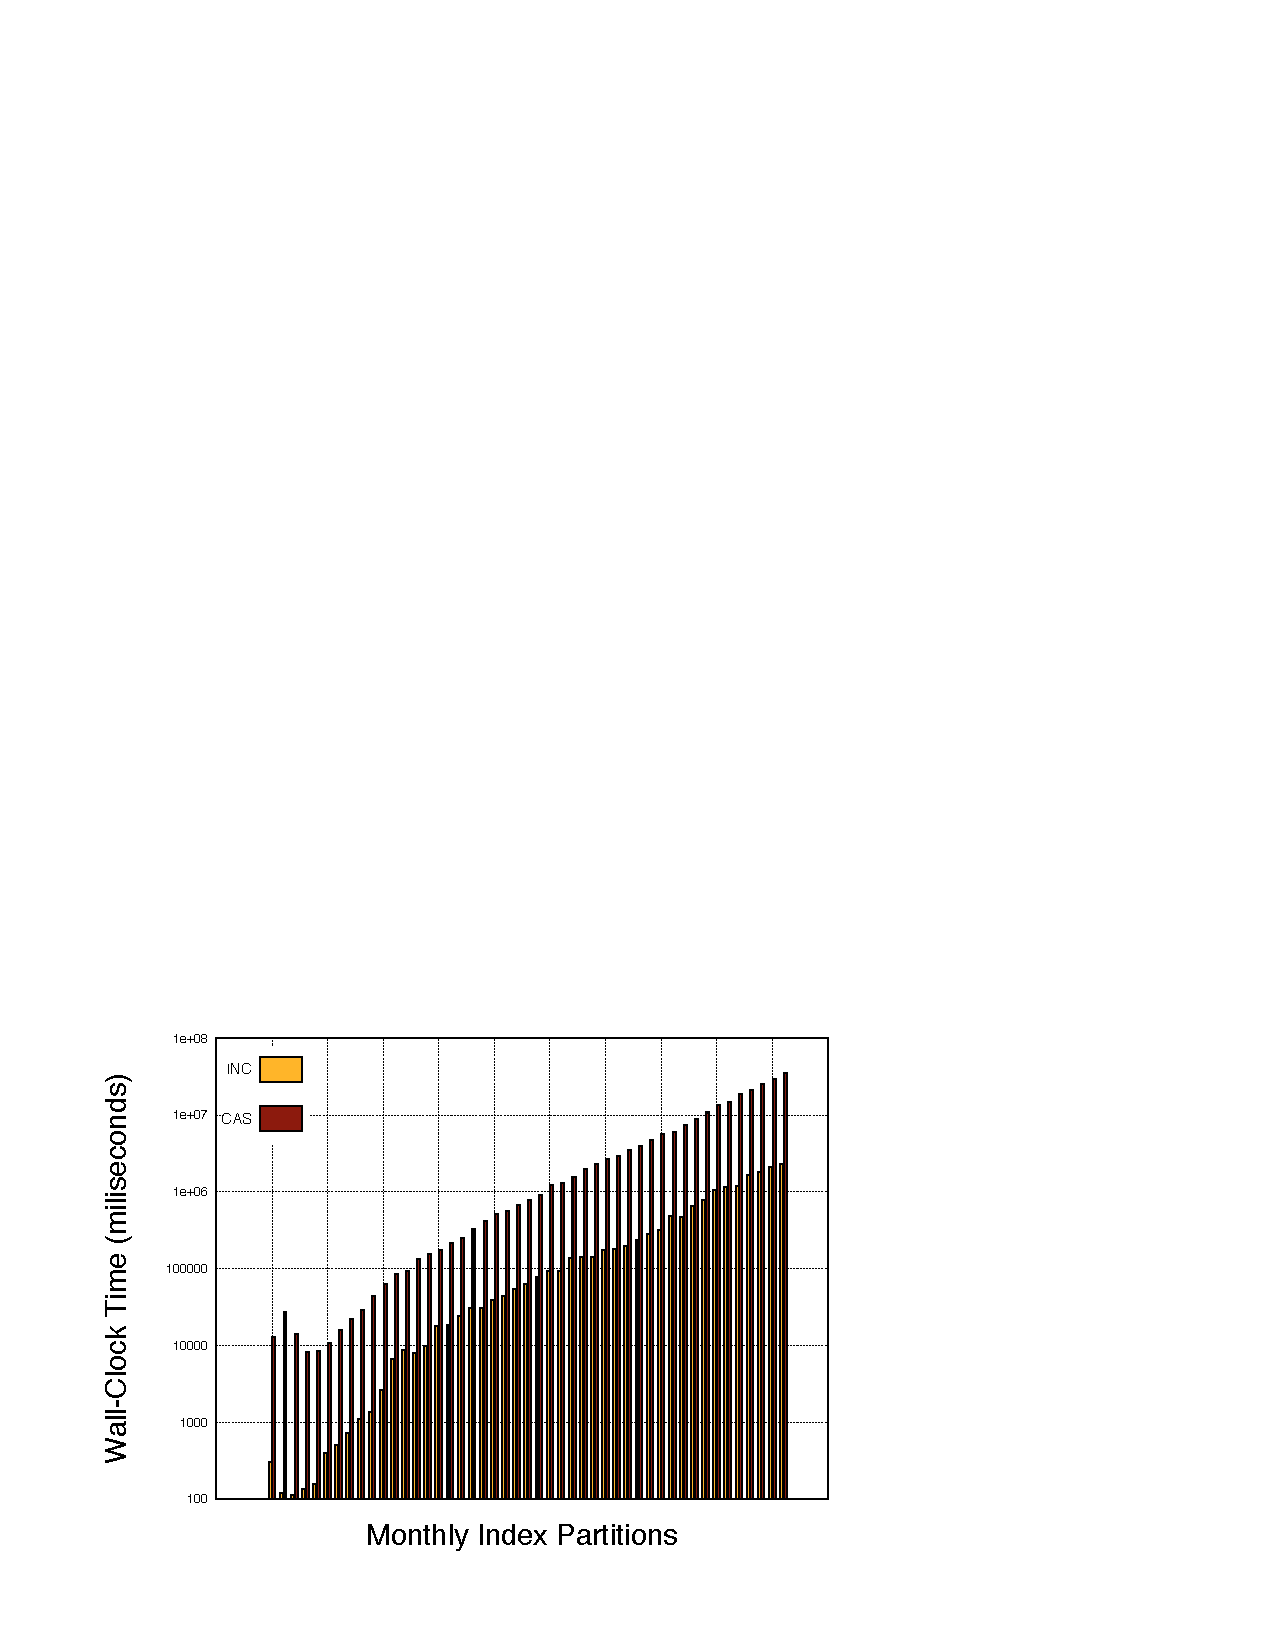
\includegraphics[width=0.3\textwidth]{plots/updates/pdfs/index_maintenance_wiki_10.pdf}}
  \subfigure[$\eta$ =
  100]{\label{fig:wiki_index_merge_100.0}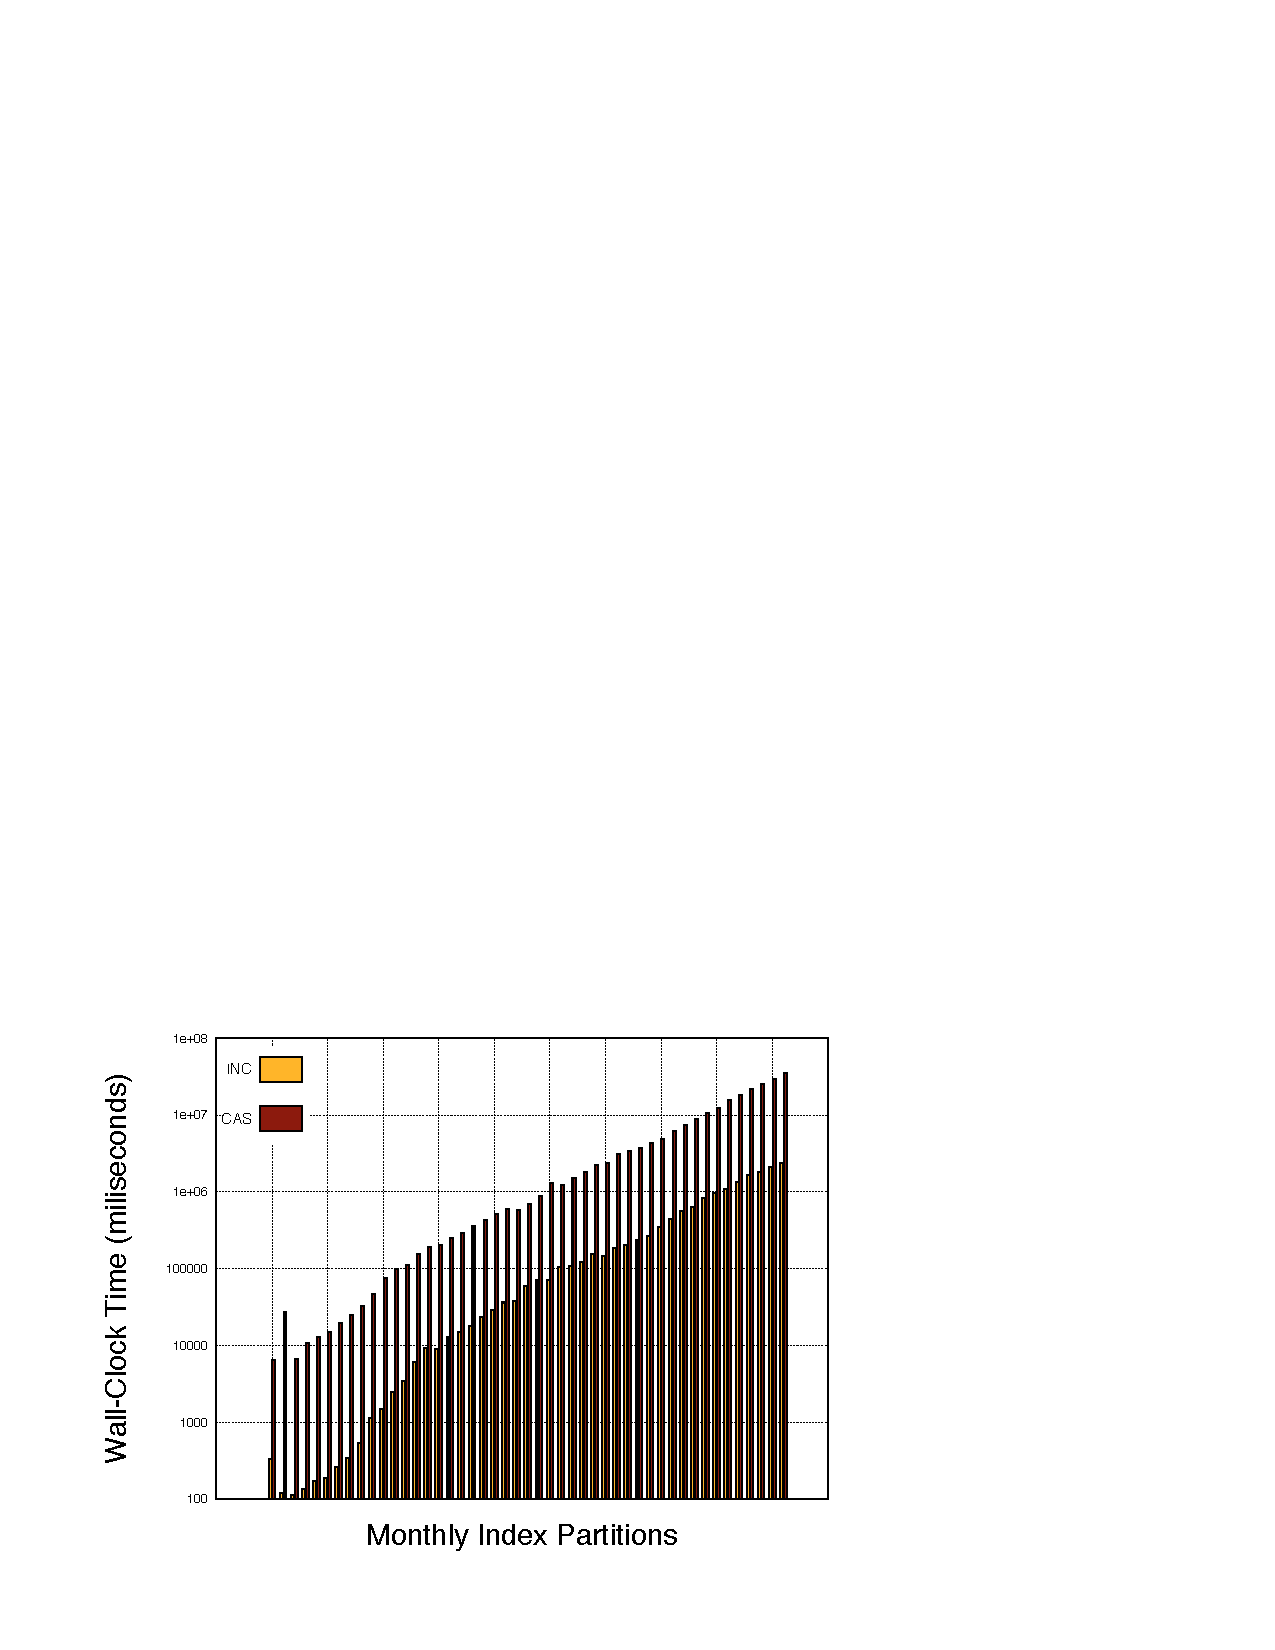
\includegraphics[width=0.3\textwidth]{plots/updates/pdfs/index_maintenance_wiki_100.pdf}}
  \subfigure[$\eta$ =
  1000]{\label{fig:wiki_index_merge_1000.0}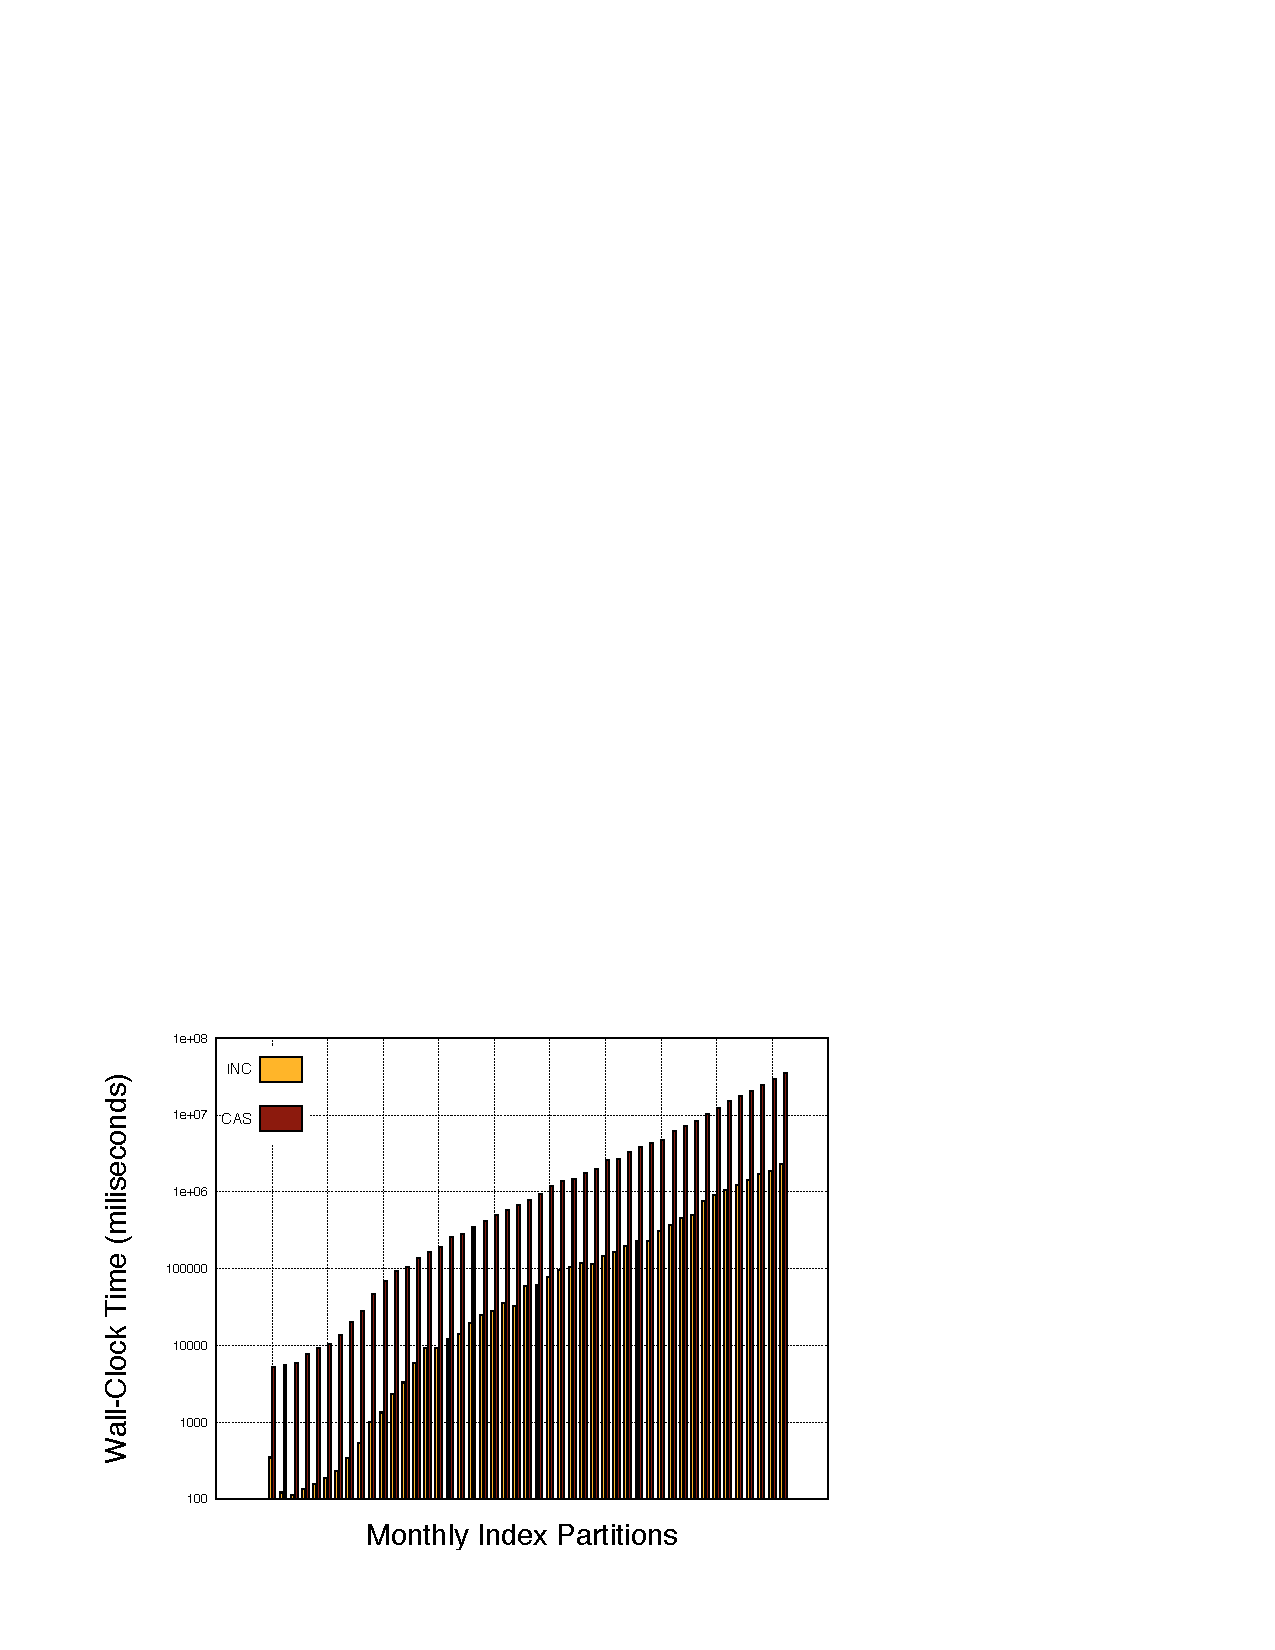
\includegraphics[width=0.3\textwidth]{plots/updates/pdfs/index_maintenance_wiki_1000.pdf}}
  \caption{Performance of index maintenance - WIKI}
  \label{fig:imwiki}
\end{figure*}

Figures~\ref{fig:imwiki} and \ref{fig:imukgov} show results of our
experiments on index maintenance with WIKI and UKGOV datasets
respectively. Note the log-scale used on the y-axis in these charts,
which represents the time-taken for the consolidated sharded index to
be built in milliseconds. It is quite evident from these charts that
the INC algorithm for maintaining the index is an order of magnitude
faster than CA. Note that for UKGOV we report maintenance times for the first seven months only which is already smaller than time taken to merge the entire index for two years using INC. This efficiency comes from two advantages that INC
enjoys over CA: first, recomputing the sharding by CA on the merged
index takes much of the time and grows as the index size grows. Since
INC does not recompute the sharding, its performance improves
significantly. Second, it does not have to decompress, merge and shard
the entire list before writing do the disk. Instead, it has to just
read two posting lists in parallel and append corresponding shards
(without decompressing), and write to the disk. From our experiments we observe that recomputation of shards accounts for an average of 45\% of the entire maintenance time. Compression and decompression take upto 15\% of the overall time but since we use 7-bit encoding for compression we expect that a more involved compression technique would only increase the maintenance time. It should be noted
that in our simulation we do not perform an append, instead we resort
to creating a new index file in each step -- incurring additional
overheads. Thus, the performance of INC can be further improved by
carefully implementing advanced index merging methods.


\begin{figure*}[!htb]
  \centering \subfigure[$\eta$ =
  10]{\label{fig:ukgov_index_merge_10.0}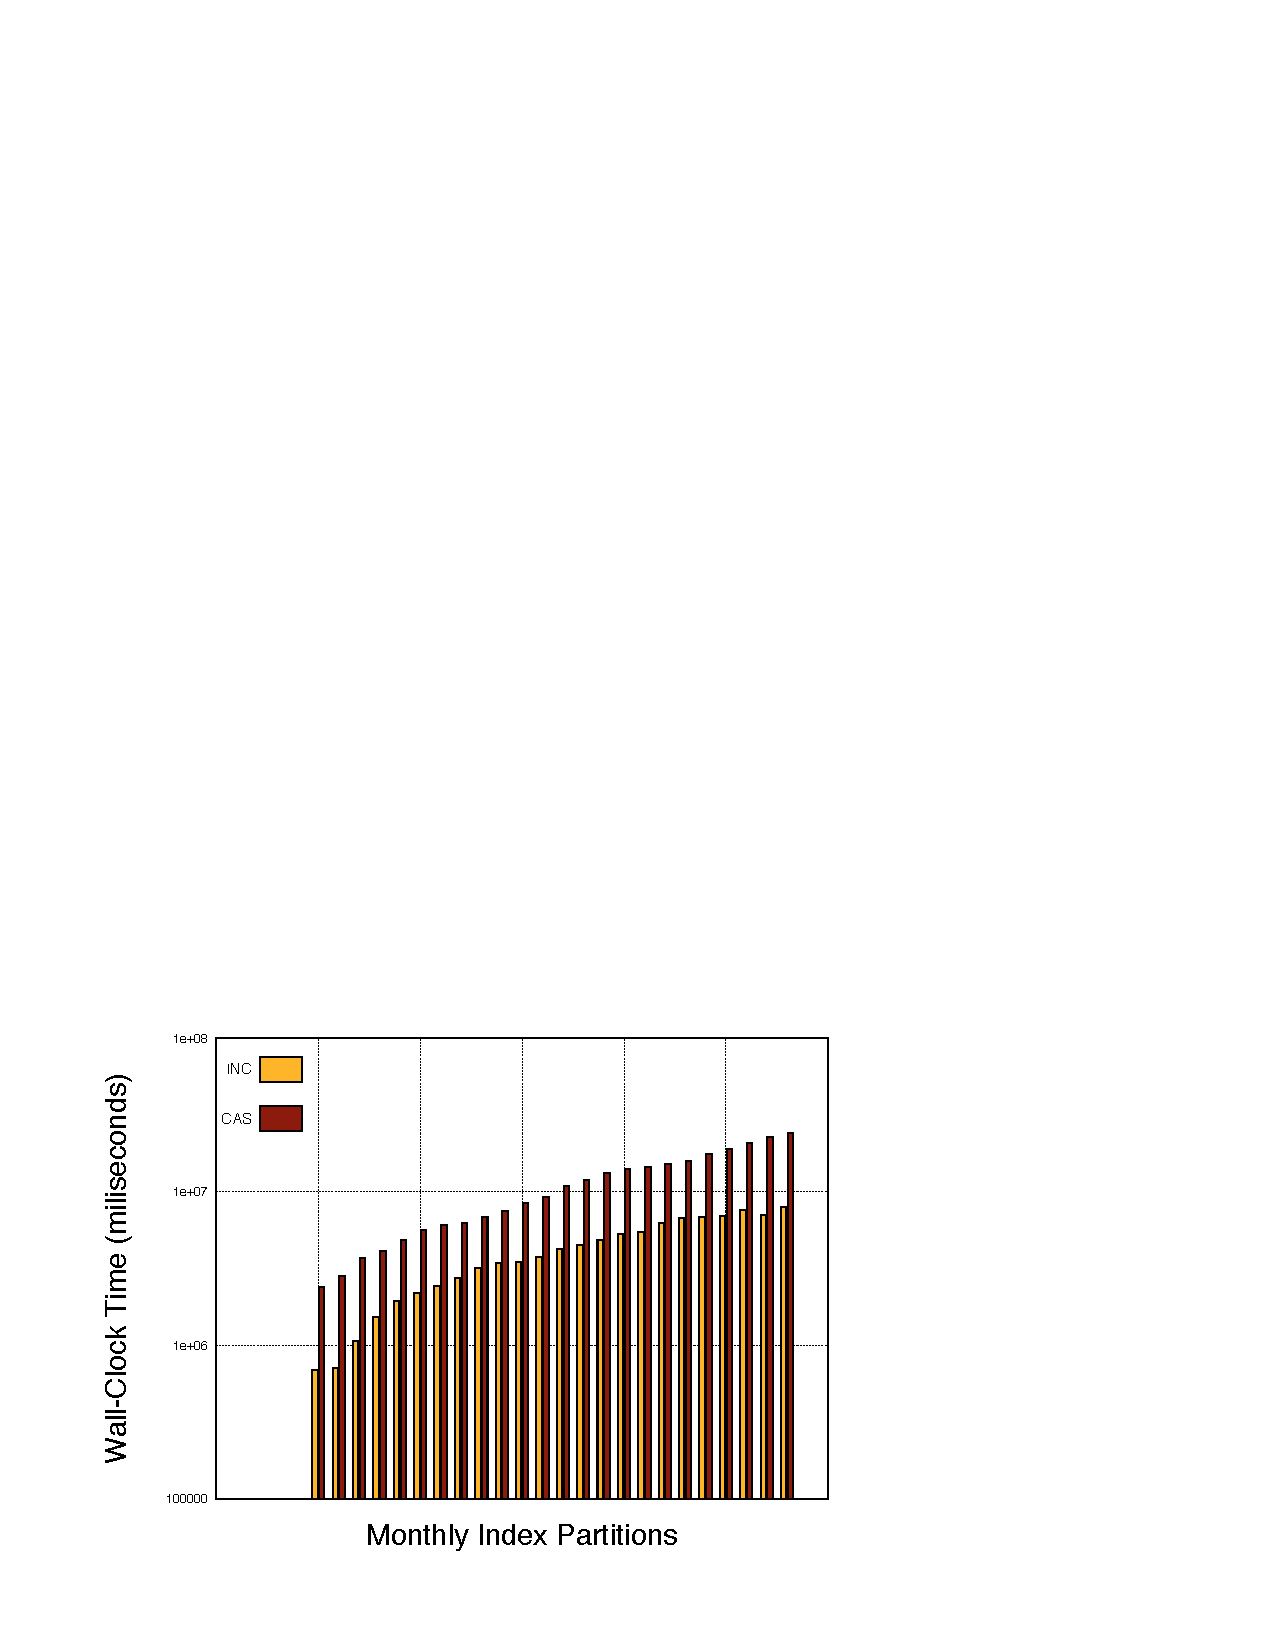
\includegraphics[width=0.3\textwidth]{plots/updates/pdfs/index_maintenance_ukgov_10.pdf}}
  \subfigure[$\eta$ =
  100]{\label{fig:ukgov_index_merge_100.0}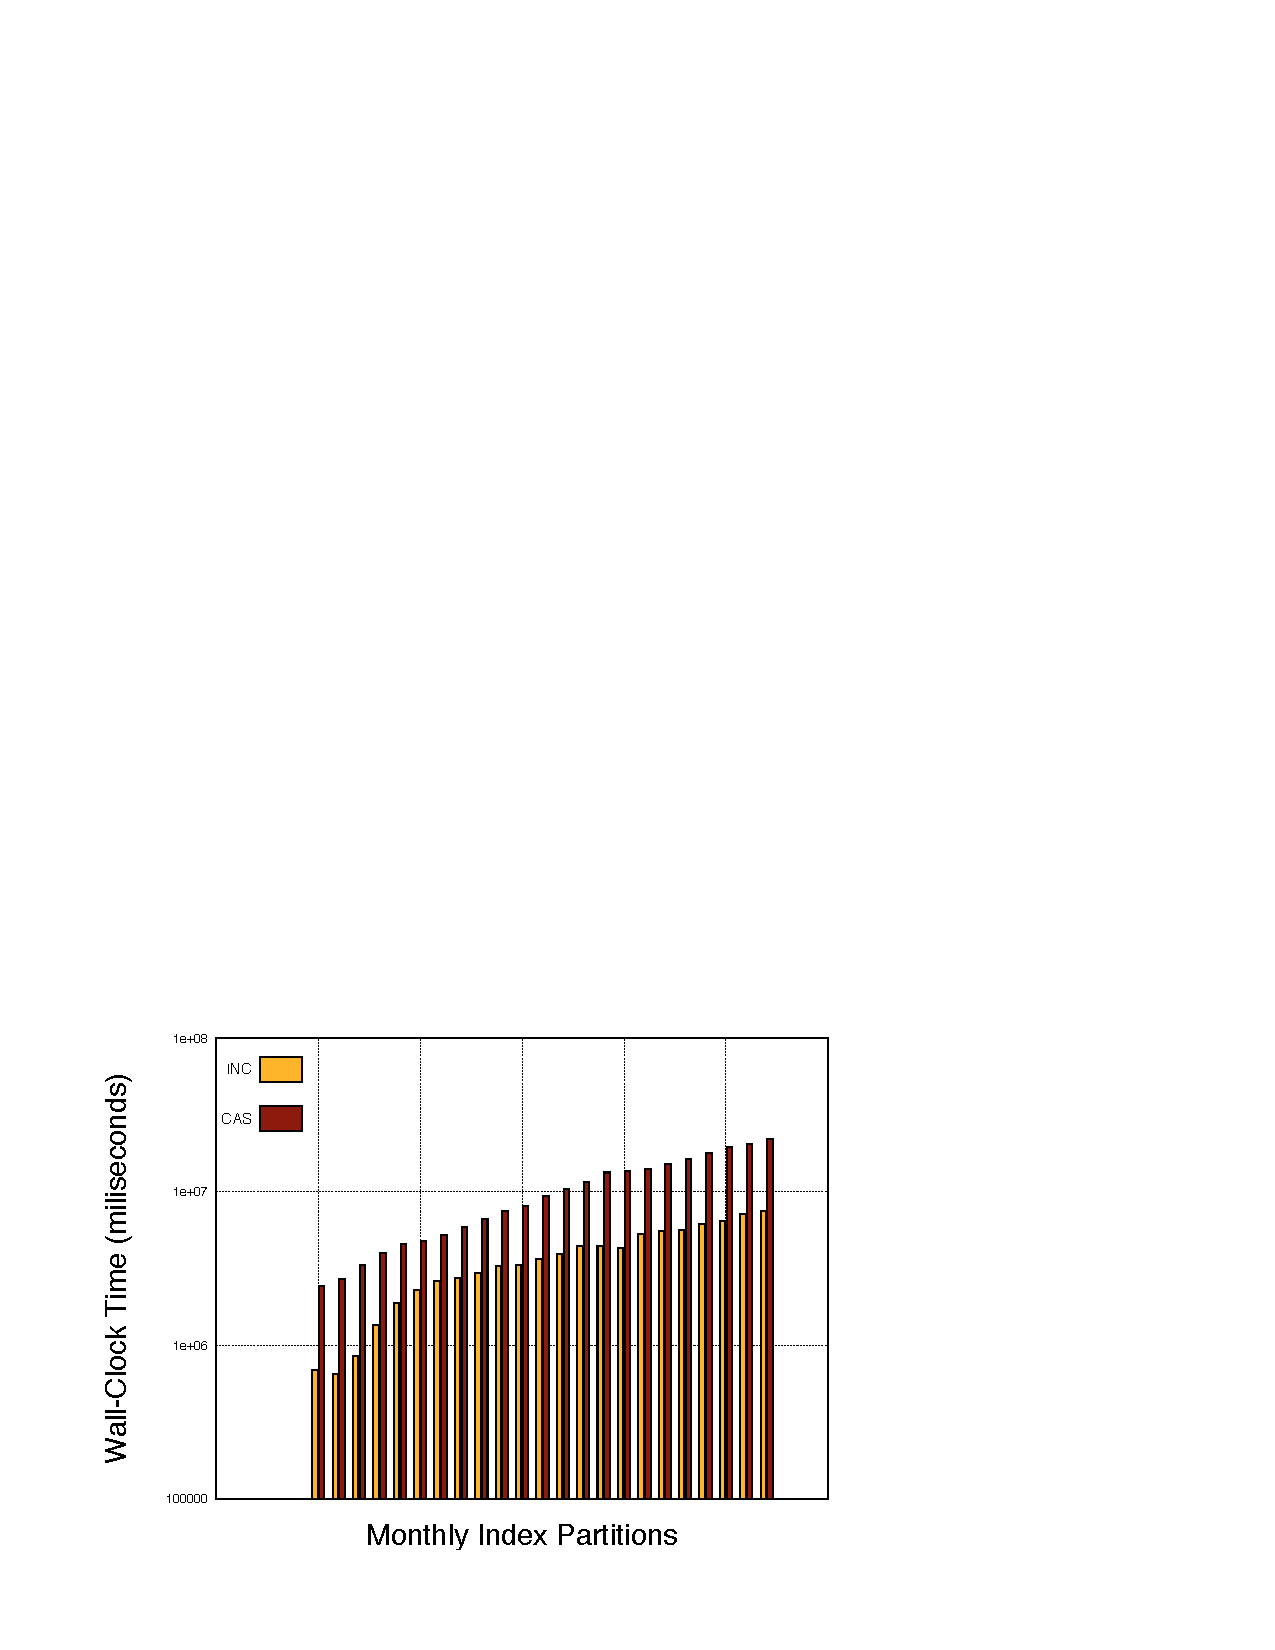
\includegraphics[width=0.3\textwidth]{plots/updates/pdfs/index_maintenance_ukgov_100.pdf}}
  \subfigure[$\eta$ =
  1000]{\label{fig:ukgov_index_merge_1000.0}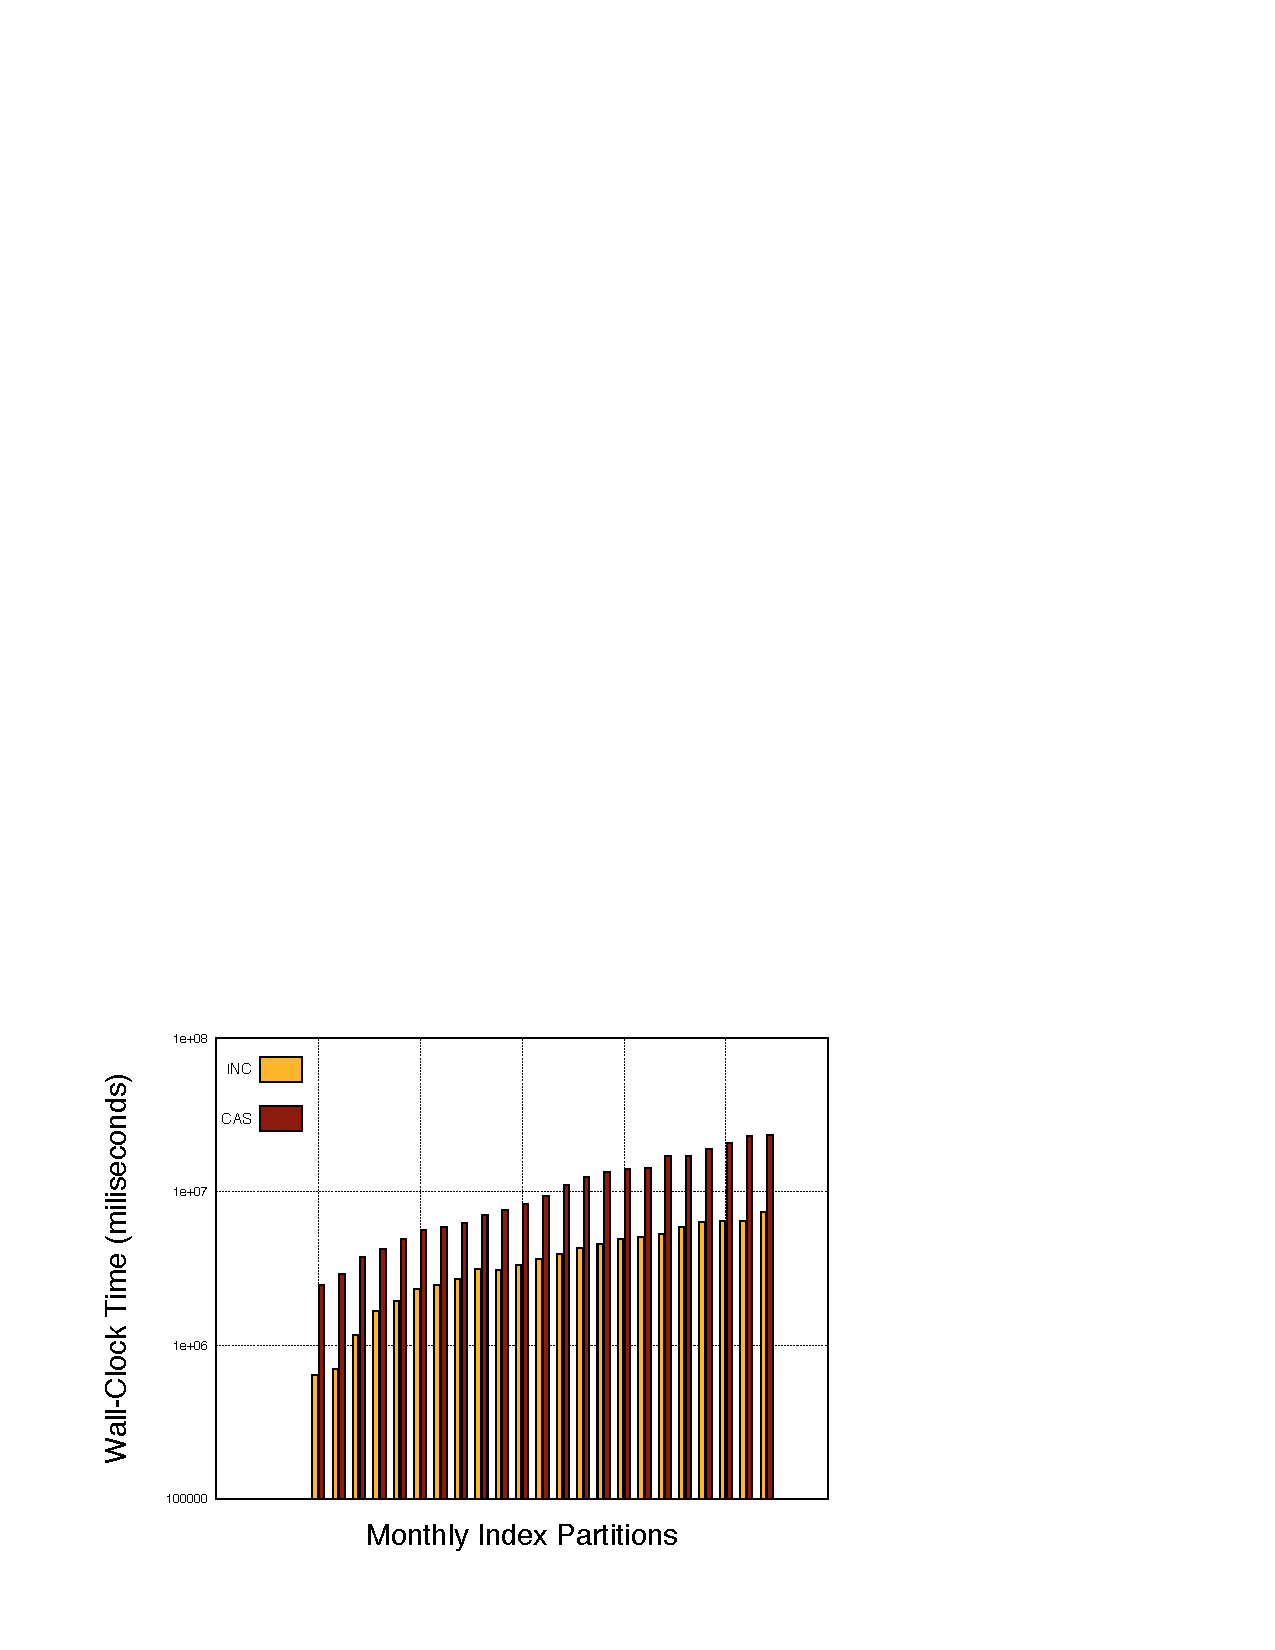
\includegraphics[width=0.3\textwidth]{plots/updates/pdfs/index_maintenance_ukgov_1000.pdf}}
  \caption{Performance of index maintenance -- UKGOV}
  \label{fig:imukgov}
\end{figure*}


\subsubsection{Effect on Query Processing}

To assess the effect of using INC for index maintenance on query
processing performance, we used the final index computed for each
dataset -- i.e., after merging the last partial index at end of 5
years in case of WIKI and after the last partial index at the end of 2
years in case of UKGOV. We compared the performance of answering
queries using this index against the query performance over a newly
created \emph{archive index} for the entire collection, sharded using
CA. Since the active index, as mentioned in ~\ref{sec:system} is
common to both INC and CA, we omitted the query processing time over
the active index from our measurements. We considered indexes obtained
using three relaxation parameter values $\eta$ = 10, 100, 1000. We
report runtimes, measured in milliseconds, averaged over queries for
three granularities of temporal predicates we considered --
\emph{week}, \emph{month} and \emph{year}, as described in
Section~\ref{sec:workload}. Results are shown in
Figures~\ref{fig:qp_wiki} and ~\ref{fig:qp_ukgov} for WIKI and UKGOV
datasets respectively.

\begin{figure*}[tb]
  \centering
  \subfigure[Week]{\label{fig:wiki_weekly_qp}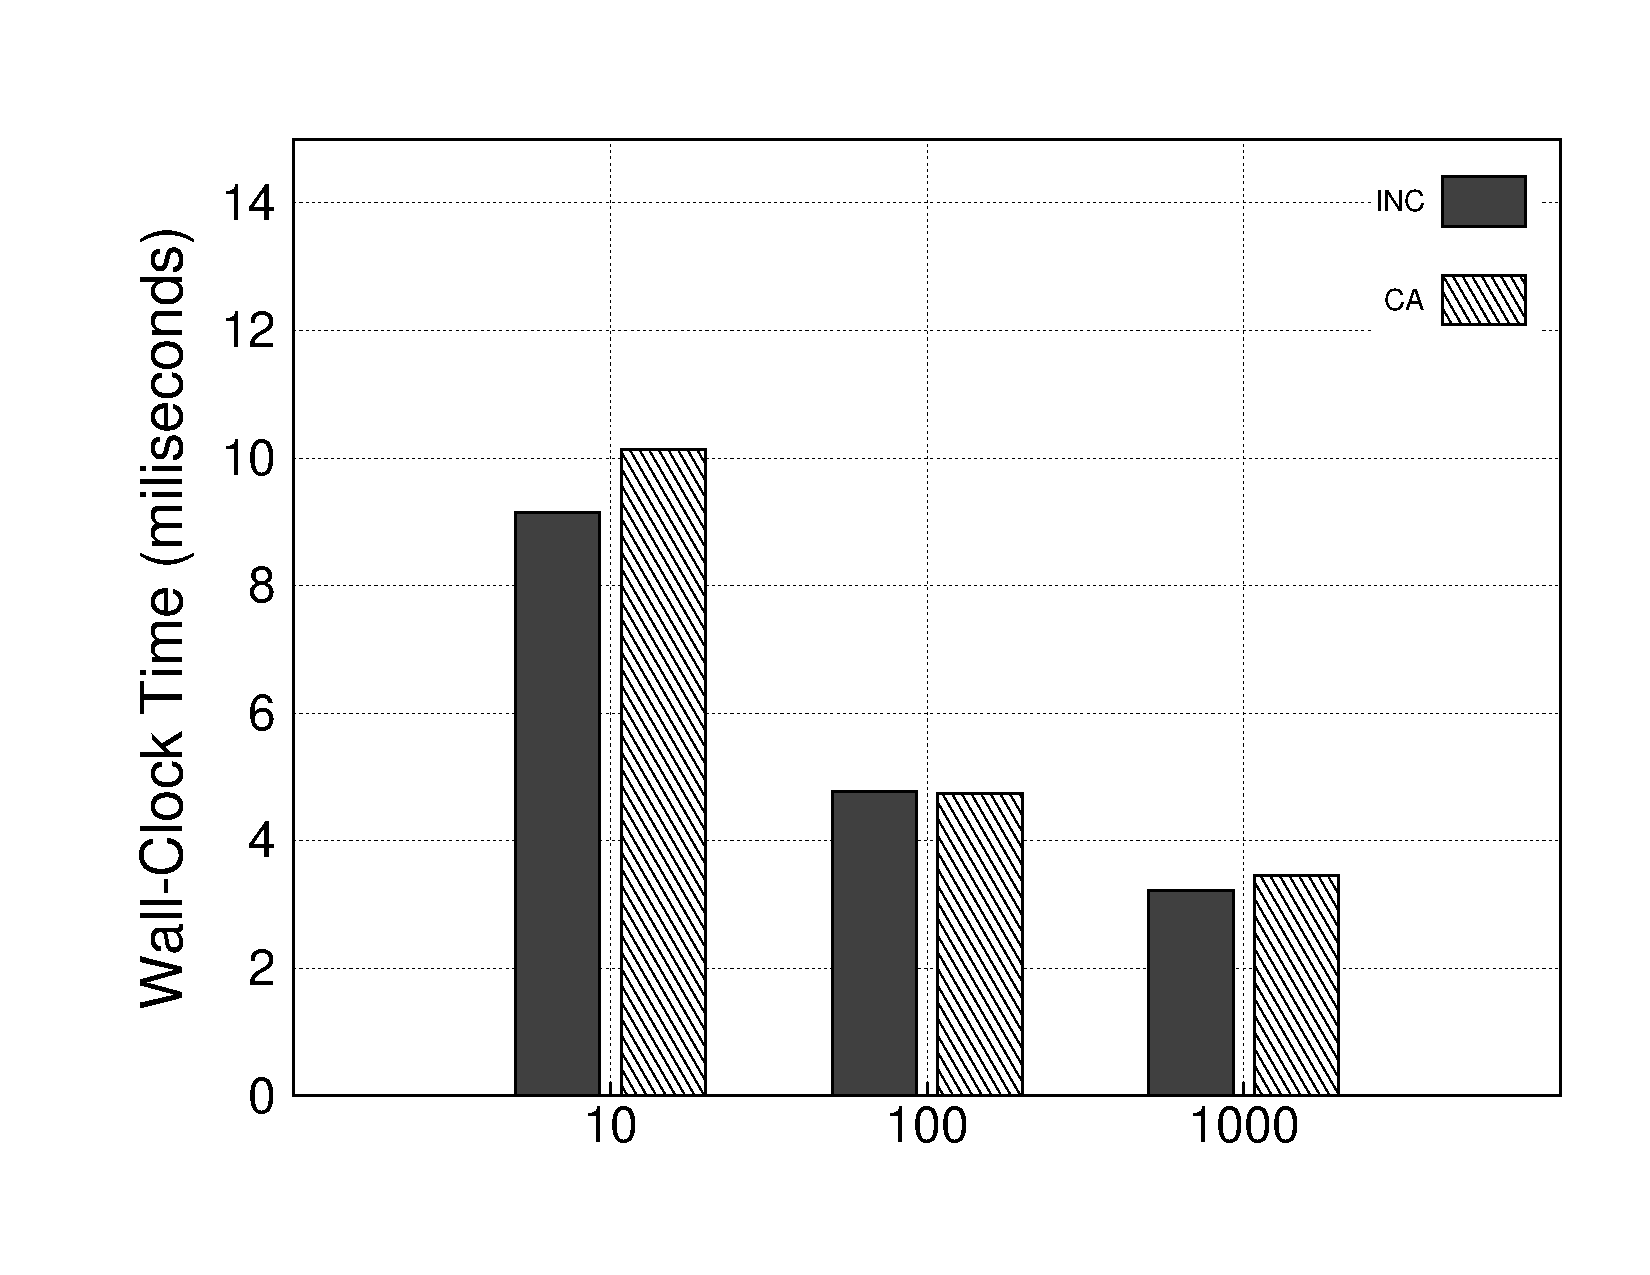
\includegraphics[width=0.3\textwidth]{plots/updates/pdfs/qp_weekly_wikipedia.pdf}}
  \subfigure[Month]{\label{fig:wiki_monthly_qp}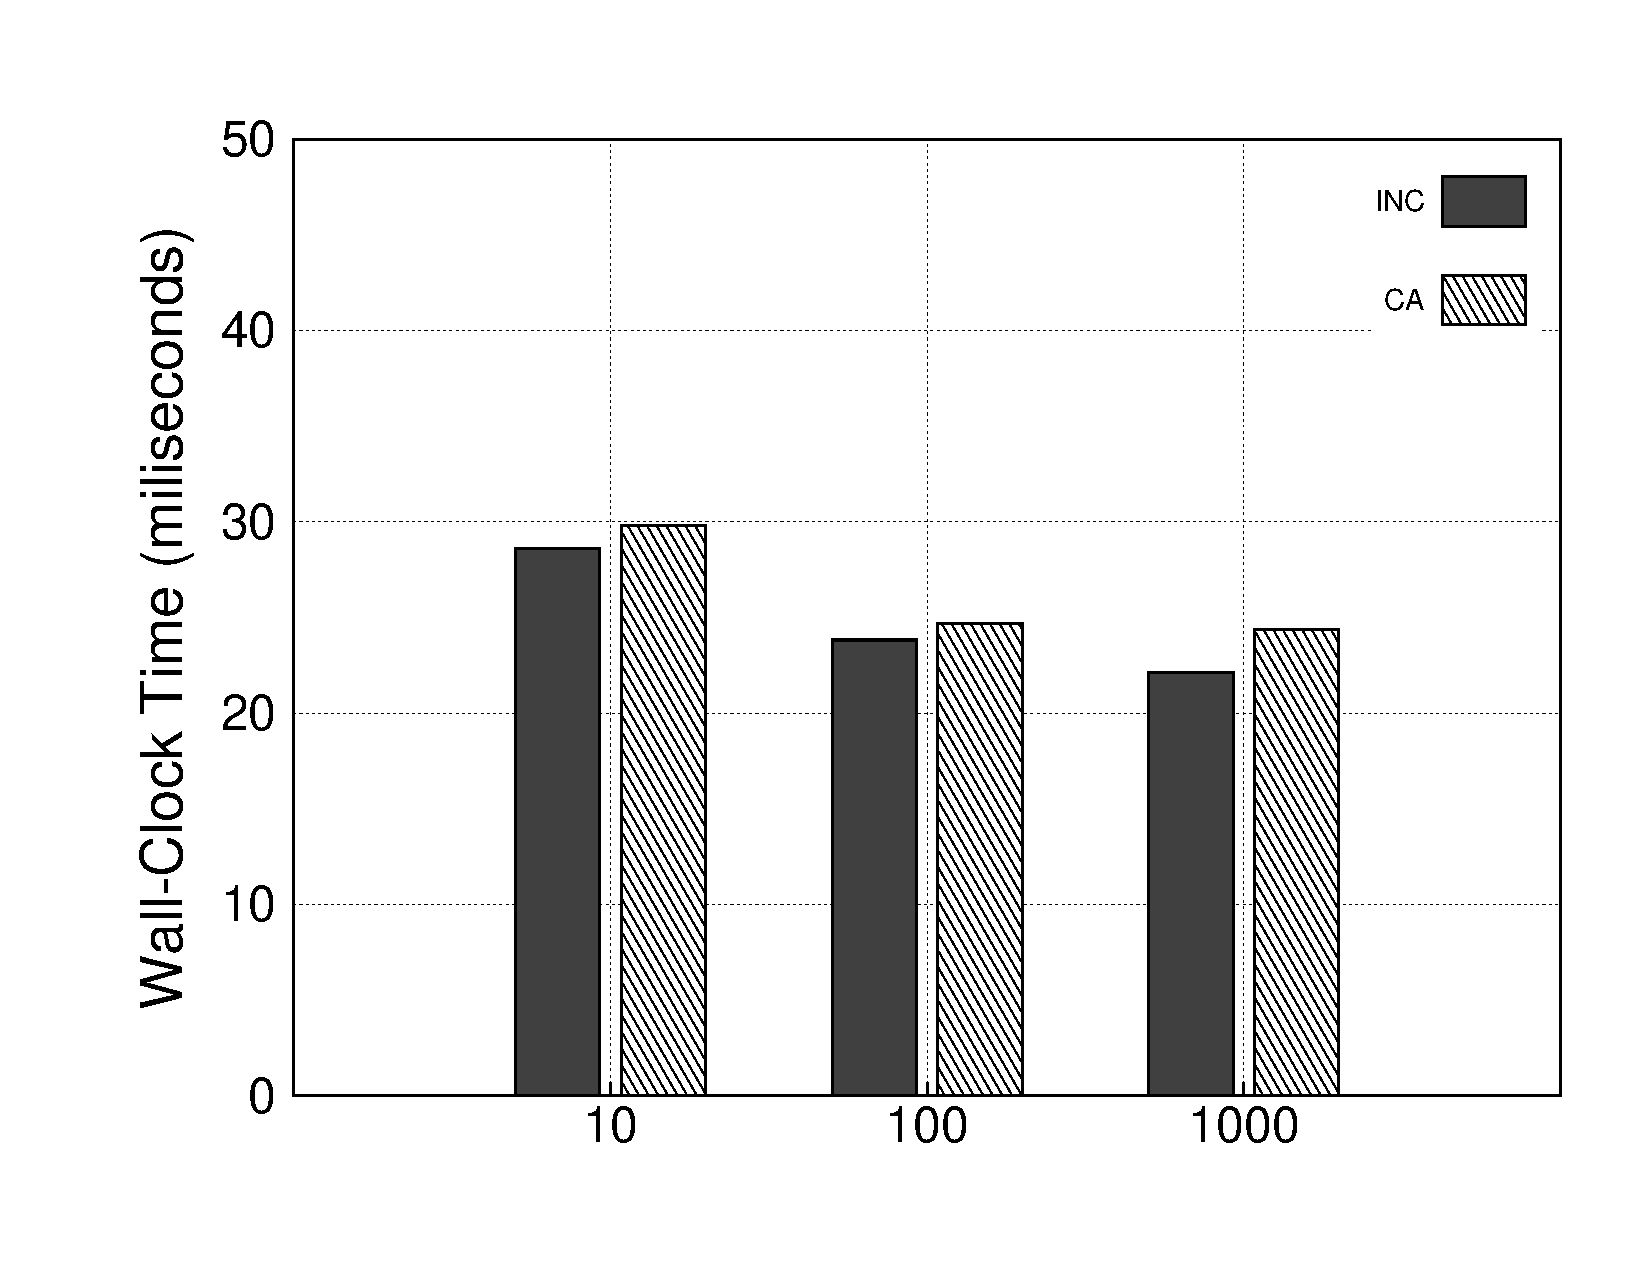
\includegraphics[width=0.3\textwidth]{plots/updates/pdfs/qp_monthly_wikipedia.pdf}}
  \subfigure[Year]{\label{fig:wiki_yearly_qp}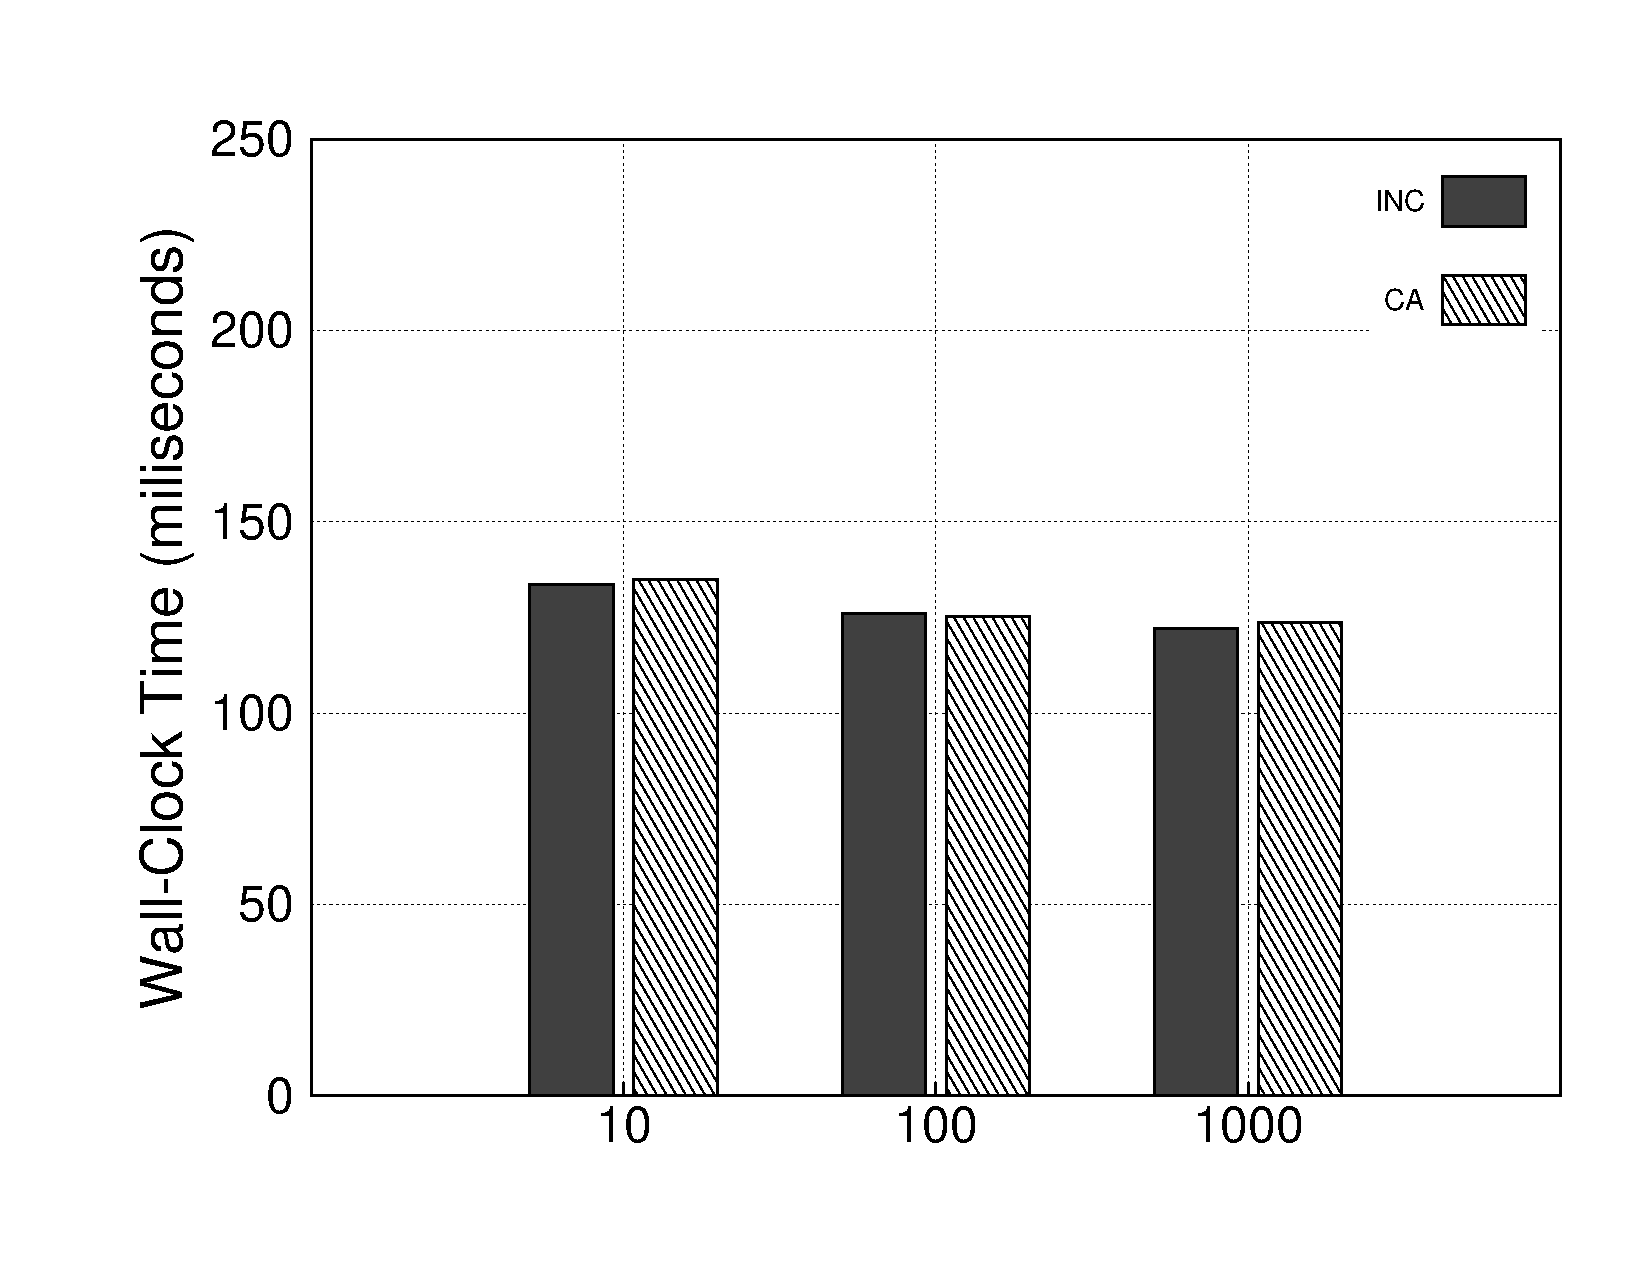
\includegraphics[width=0.3\textwidth]{plots/updates/pdfs/qp_yearly_wikipedia.pdf}}
  \caption{Query processing performance with varying granularity of
    temporal predicate -- WIKI}
  \label{fig:qp_wiki}
\end{figure*}
\begin{figure*}[tb]
  \centering
  \subfigure[Week]{\label{fig:ukgov_qp_week}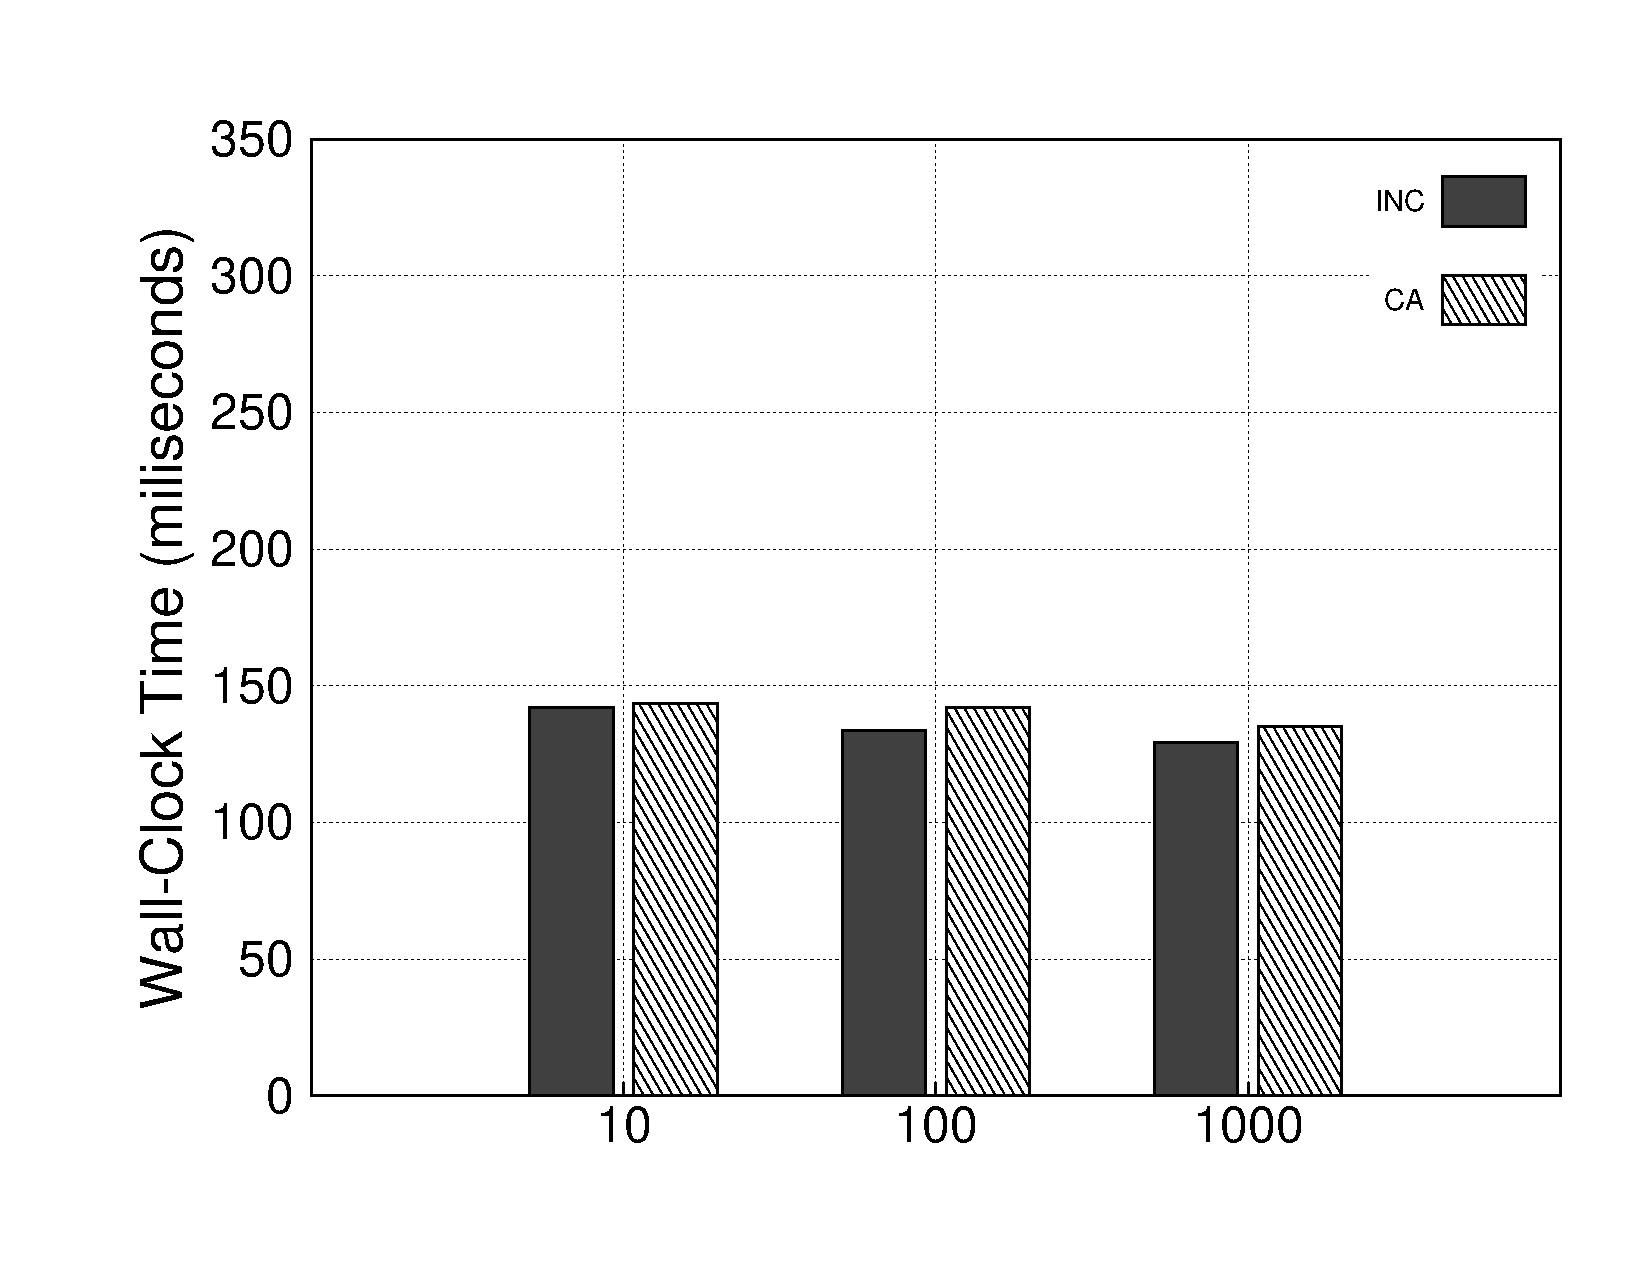
\includegraphics[width=0.3\textwidth]{plots/updates/pdfs/qp_weekly_ukgov.pdf}}
  \subfigure[Month]{\label{fig:ukgov_qp_month}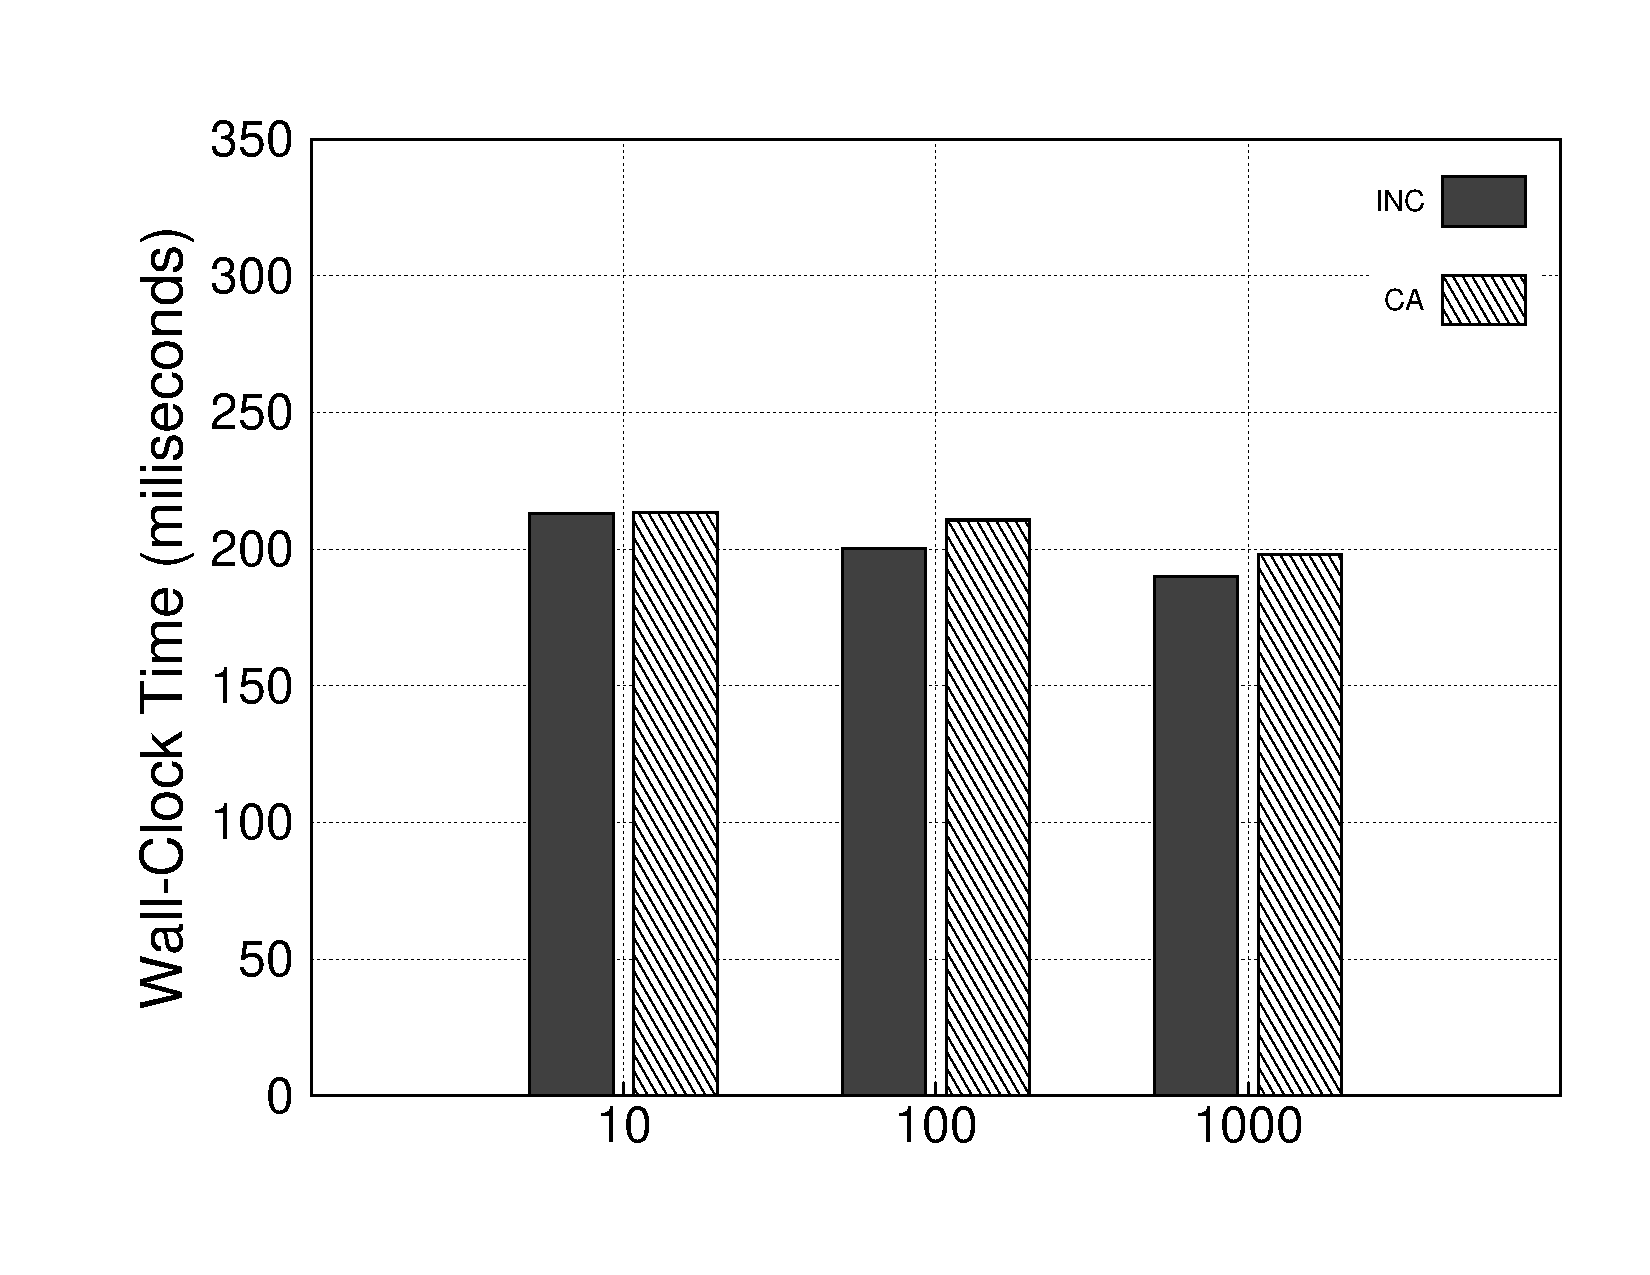
\includegraphics[width=0.30\textwidth]{plots/updates/pdfs/qp_monthly_ukgov.pdf}}
  \subfigure[Year]{\label{fig:ukgov_qp_year}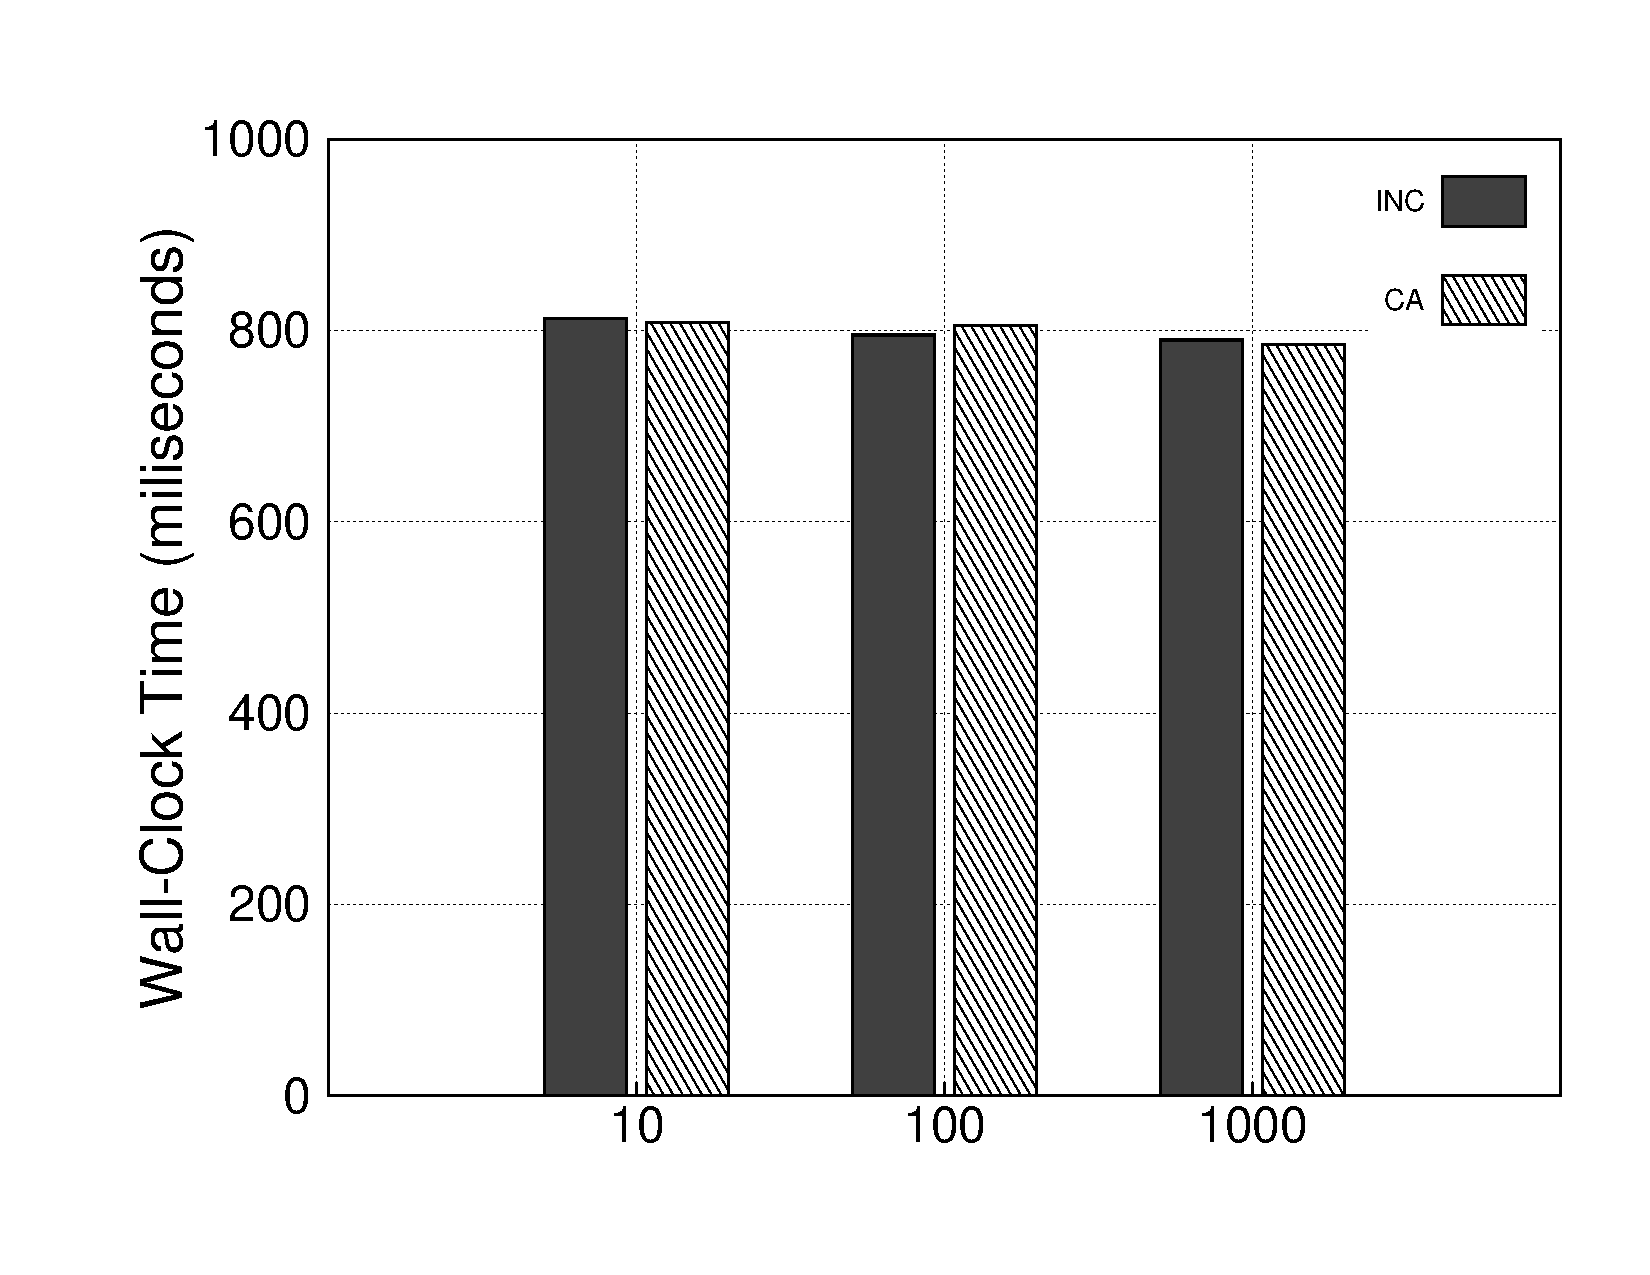
\includegraphics[width=0.30\textwidth]{plots/updates/pdfs/qp_yearly_ukgov.pdf}}
  \caption{Query processing performance with varying granularity of
    temporal predicate -- UKGOV}
  \label{fig:qp_ukgov}
\end{figure*}

As one can observe from these charts, the sharded index generated
using INC compares quite favorably with the combined sharded index
computed using CA. This behavior is consistent across all the
granularities of temporal predicate for all values of $\eta$
parameter. In some small number of cases, the performance of INC is
slightly better than that of CA, and is never worse. Further, we also
compared the average number of shards generated by both the algorithms
with different values of $\eta$. These results are summarized in
Table~\ref{tab:shard_dist}. As these results show, using INC in most
cases generates fewer number of shards on average for each posting
list, reducing the number of random accesses required during query
processing. So, when the underlying storage system has high cost of
random accesses, then it seems more beneficial to query processing
performance to use INC to maintain the index than using CA.

% We firstly observe that with the increase in the relaxation
% parameter the overall number of shards per term decreases (see
% Table~\ref{tab:shard_dist}), reducing the number of random accesses
% which have to be performed during query processing. Consequently,
% query processing times for incremental sharding reduce from 57ms to
% 49ms (WIKI) and 391ms to 369ms in UKGOV. Incremental sharding
% consistently performs slightly better than CAS in both
% datasets, %In Wikipedia, incremental sharding is XXX\% better than CAS for smaller $\eta$ while the difference increases/decreases to XXX\% for $\eta = 1000$. In UKGOV, the difference is very small and in fact CAS performs better for a relaxation parameter of 10.
% and as we allow for more relaxations, the difference in query
% processing times increases. Detailed results are shown in
% Figures~\ref{fig:qp_wiki} and ~\ref{fig:qp_ukgov}.

% 1) Difference get smaller as the value of relaxation parameter
% increases. This is because the difference in the number of shards
% keeps reducing (check with new numbers) 2) Any distinguishing factor
% between UKGOV and WIKI, any new insights ? Any expected behavior
% based on typical nature of these collections ?  3) Incremental
% sharding is more restrictive and hence more number of shards than
% CAS.  4) Rewards long time interval query which typically involve
% larger seq. reads (check claim)

% \begin{table}[htb]
% \begin{tabular}{l @{ } c c c @{  } c c c }
% \toprule
% &\multicolumn{3}{c}{Incremental Sharding}&\multicolumn{3}{c}{Cost-Aware Sharding}\\
% &10&100&1000&10&100&1000\\
% \cmidrule{2-4} \cmidrule{3-7}
% WIKI&23.37&13.32&5.83&32.83&11.41&4.42\\
% UKGOV&10.93&6.84&4.14&13.16&10.35&4.79\\
% \bottomrule
% \end{tabular}
% \caption{Average number of shards per term}
% \label{tab:shard_dist}
% \end{table}



\begin{table}[tb]
  \center
  \begin{tabular}{l @{\hspace{0.2cm}} l @{\hspace{0.3cm}} c @{\hspace{0.3cm}} c}
    \toprule
    & & \multicolumn{2}{c}{\bf Sharding }\\
    \cmidrule{3-4}
    Dataset &$\eta$ & INC & CA\\
    \midrule
    \multirow{3}{*}{\bf WIKI} & $10$ & 23.37 & 32.83 \\
    & $100$ & 13.32 & 11.41 \\
    & $1000$ & 5.83 & 4.42 \\
    \\
    \multirow{3}{*}{\bf UKGOV}& $10$ & 10.93 & 13.16 \\
    & $100$ & 6.84 & 10.35 \\
    & $1000$ & 4.14 & 4.79 \\
    \bottomrule
  \end{tabular}
  \caption{Average number of shards per term}
  \label{tab:shard_dist}
\end{table}

% Related Work
\section{Related Work}
\label{sec:related-work}

We now put our work in context with existing research. This can be
categorized into (a) work on maintaining inverted indexes when faced
with changes in the document collection and (b) approaches that make
search aware of temporal information associated with documents. No
work, to the best of our knowledge, has been done at the intersection
of the two categories.

Given that the construction of inverted indexes is well understood and
can easily be parallelized, one existing maintenance strategy has been
to rebuild the index periodically. Returning stale query results, most
of the time, is an obvious disadvantage of this approach. For a long
time, though, this has been the approach taken by major search engines
on the Web. Only lately, Peng et al.~\cite{Peng:2010fk} have addressed
the issue of handling updates in web-scale indexes. Instead of
rebuilding the index, Lester et al.~\cite{Lester:2006ly} suggest to
collect updates in an in-memory index that is then merged, from time
to time to amortize costs, with a disk-resident inverted index. This
merge can either be performed in-situ, thus modifying posting lists at
their current location, or by storing entirely new posting lists. A
hybrid approach that chooses between these alternatives is described
by B\"uttcher et al.~\cite{Buttcher:2008fk}. Guarajada and
Kumar~\cite{Gurajada:2009vn} can be seen as another extension that
leverages query logs to determine terms whose posting lists mandate
eager maintenance. In a spirit similar to log-structured
methods~\cite{ONeil:1996fk}, Lester et al.~\cite{Lester:2008qf}
propose to keep multiple indexes of geometrically increasing size and
merge them, when they overflow, in a rolling manner. Query results
reflecting the current state of the document collection can be
obtained in these approaches by executing queries both on in-memory
and disk-resident indexes. For more detailed discussions of inverted
index maintenance, we refer to the recent textbooks by B\"uttcher et
al.~\cite{BuettcherCC10} and Manning et al.~\cite{manning:2008}, as
well as, the survey by Zobel and
Moffat~\cite{DBLP:journals/csur/ZobelM06}.

Constructing indexes for (versioned) document collections with a high
degree of redundancy has been an active area of research lately. Anick
and Flynn~\cite{DBLP:conf/sigir/AnickF92}, as the earliest approach,
applies techniques from version-control systems to a text index. Zhang
and Suel~\cite{Zhang:2007fk} propose a two-level index that avoids
repeatedly indexing redundant content. Herscovici et
al.~\cite{DBLP:conf/ecir/HerscoviciLY07} employ a sequence-alignment
formulation to address the same problem. Berberich et
al.~\cite{kberberi:sigir2007} present the idea of time-travel text
search, incorporating temporal predicates into text search, and
describe a vertically partitioned (or, sliced) inverted index to
support it efficiently. Anand et al.~\cite{aanand:sigir2011}, as the
work that our methods build upon, show that time-travel text search
can be supported equally efficiently by building a horizontally
partitioned (or, sharded) inverted index. He et
al.~\cite{DBLP:conf/cikm/HeYS09,DBLP:conf/cikm/HeZS10} have focused on
improving compression techniques for inverted indexes on versioned
document collections. As a final note, the problem of indexing and
querying data with associated temporal information has been studied
intensively in the database community -- a survey of existing
approaches is given by Salzberg and Tsotras~\cite{salzberg:csur1999}
present. Becker et al.~\cite{Becker:1996aa}, being based on the
$B^{+}$-Tree, and Muth et al.~\cite{Muth2000}, as a log-structured
method inspired by the LSM-Tree~\cite{ONeil:1996fk}, are two database
approaches that explicitly deal with updates.

% Conclusions

\section{Conclusions}
\label{sec:conclusions}

This paper presented incremental sharding, an efficient maintenance
technique for indexes in web archives. It uses only cheap append
operations to add newly arrived versions to the existing index. It can
be smoothly integrated into a search engine for both live and archived
documents. Experiments demonstrated that the technique is an order of
magnitude more efficient than recomputing the index.

Our future work will focus on an full-fledged implementation of our
proposed system. We will further study the influence of different
techniques for inverted list maintenance.

